%---------------------------------------------------------------------
%   毕业论文 LaTeX 完整初稿
%--------------------------------------------------------------------

\documentclass[a4paper,12pt]{report}
\usepackage{geometry} 
\geometry{a4paper,left=2.5cm,right=2.5cm,top=2.54cm,bottom=2.54cm}
\usepackage[fontset=none]{ctex} % 关闭 ctex 默认 mac 字体集（STSong/STHeiti），改用自定义字体
\usepackage{xeCJK}
% 字体方案 B：使用“思源宋体/思源黑体（简体）”以获得完整字重（含粗体），避免 STSong/STHeiti 字形缺失告警
% （你已下载 SourceHanSansSC/SourceHanSerifSC 并安装到“字体册”后）重启 VSCode 再编译
\xeCJKsetup{AutoFakeBold=true, AutoFakeSlant=true} % 若某字重未被系统识别，仍可用伪粗体兜底
\setCJKmainfont{Source Han Serif SC}
\setCJKsansfont{Source Han Sans SC}
% 解决 xeCJK “Unknown CJK family \CJKttdefault” 的提示：指定等宽字体
%（若你更偏好系统等宽字体，也可改为 Menlo）
\setCJKmonofont{Source Han Sans SC}
% 让 \songti/\heiti/\kaishu/\fangsong 等字体命令切换到思源字体
\setCJKfamilyfont{song}{Source Han Serif SC}
\setCJKfamilyfont{hei}{Source Han Sans SC}
\setCJKfamilyfont{kai}{Source Han Serif SC}
\setCJKfamilyfont{fang}{Source Han Serif SC}
% 注意：fontset=none 时 ctex 可能不预定义这些命令，因此用 \providecommand 防御
\providecommand{\songti}{}
\providecommand{\heiti}{}
\providecommand{\kaishu}{}
\providecommand{\fangsong}{}
\renewcommand{\songti}{\CJKfamily{song}}
\renewcommand{\heiti}{\CJKfamily{hei}}
\renewcommand{\kaishu}{\CJKfamily{kai}}
\renewcommand{\fangsong}{\CJKfamily{fang}}
\usepackage{setspace}
\usepackage{fancyhdr}
\usepackage{graphicx}
\usepackage{adjustbox} % scale tables down only when needed (avoid resizebox upscaling)
\usepackage{tikz}
\usetikzlibrary{arrows.meta,positioning,shapes.geometric}
\usepackage{array}
\usepackage{titlesec}
\usepackage{titletoc}
\usepackage{amsmath}
\usepackage{amsthm}
\usepackage{amsfonts}
\usepackage{booktabs}
\usepackage{multirow}
\usepackage{hyperref}
\hypersetup{hidelinks,pdfborder={0 0 0}}
\hypersetup{hidelinks,pdfborder={0 0 0}}
\usepackage{caption}
\usepackage{fvextra} % for breakable verbatim (avoid overfull lines in prompts)
\usepackage{makecell} % for multi-line cells in baseline tables
\usepackage{zhnumber}
\usepackage{threeparttable}
\usepackage{chngcntr}
\usepackage{float}

% 参考文献（biblatex；与 natbib 命令兼容）
% 目标：文内为“作者—年份”格式（如：Schumpeter（1911）或（Schumpeter，1911）），
%      文末参考文献为带编号的条目（如：[1] ...），并按作者字母顺序排序。
% 编译顺序：XeLaTeX -> Biber -> XeLaTeX -> XeLaTeX
\usepackage[
  backend=biber,
  style=references/gb7714-2015, % 文末参考文献：编号体例
  citestyle=authoryear,         % 文内引用：作者—年份体例
  gbnamefmt=none,
  gbpub=false,               % 作者名不要全大写
  giveninits=true,              % 名用首字母缩写
  uniquename=init,              % 避免与 gb7714 默认选项冲突
  seconds=true,                 % 避免 gb7714 的 eventdate=iso 相关警告
  sorting=nyt,
  maxcitenames=1,
  mincitenames=1,
  maxbibnames=99,
  natbib=true,
  sortcites=false
]{biblatex}
\addbibresource{references/reference.bib}

% 自定义排序：presort > sortkey > year > title
\DeclareSortingTemplate{presort}{
  \sort{
    \field{presort}
  }
  \sort{
    \field{sortkey}
  }
  \sort{
    \field{year}
  }
  \sort{
    \field{title}
  }
}

% 改为使用presort排序
\ExecuteBibliographyOptions{sorting=presort}

% 行内引用标点（中文括号 + 中文逗号/分号）
% 注意：不要依赖 \addpunct/\bibcomma 等内部命令（在 gb7714 样式组合下可能不存在或不可用）。
\DeclareDelimFormat{nameyeardelim}{，}%
\DeclareDelimFormat{multicitedelim}{；}%
\renewcommand*{\mkbibparens}[1]{（#1）}

% 让“参考文献”以一级标题形式进入目录（不编号）
\defbibheading{bibintoc}[参考文献]{%
  \chapter*{#1}%
  \addcontentsline{toc}{chapter}{#1}%
}
% 脚注设置：圆圈内加数字，每页重新编号
\usepackage{pifont}
\renewcommand{\thefootnote}{\ding{\numexpr171+\value{footnote}}}
\usepackage{perpage}
\MakePerPage{footnote}
% 参考文献表：gb7714-2015 样式默认即为半角标点；此处不再强行重定义，避免触发未定义命令

% 页面设置
\setlength{\baselineskip}{22pt}
\setlength{\headheight}{15pt}
\pagestyle{plain} % 按照要求删除页眉

% 标题与计数器设置
% 图表编号按全文连续编号（不按章重置）
% 取消“按章编号”的前缀，避免出现“图 三、.1 / 表三、.2”
\counterwithout{figure}{chapter}
\counterwithout{table}{chapter}
\counterwithout{equation}{chapter}
% 图表编号显示为 1,2,3...
\renewcommand{\thefigure}{\arabic{figure}}
\renewcommand{\thetable}{\arabic{table}}
% 公式编号显示为 (1),(2)...（amsmath 默认会自动加括号，所以这里不要再手写括号）
\renewcommand{\theequation}{\arabic{equation}}
\titleclass{\chapter}{straight}
\renewcommand\thesection{（\zhnum{section}）}
\renewcommand\thesubsection{\arabic{subsection}.}
\renewcommand \thechapter {\zhnum{chapter}、}
\titleformat{\chapter}{\centering\zihao{4}\songti\bfseries}{\thechapter}{1em}{}
\titleformat{\section}{\zihao{-4}\songti\bfseries}{\thesection}{1em}{}
\titleformat{\subsection}{\zihao{-4}\songti}{\thesubsection}{1em}{}
% 二级及以下标题取消与上下文之间的额外空白
\titlespacing*{\section}{0pt}{0pt}{0pt}
\titlespacing*{\subsection}{0pt}{0pt}{0pt}

% 图表题：显示为“图1”“表1”（无标点、无空格）
\renewcommand{\figurename}{图}
\renewcommand{\tablename}{表}
% “序号与标题之间不加标点，只空两格”：用 \quad 作为间距近似“两格”
\captionsetup[figure]{labelsep=quad, justification=centering, singlelinecheck=false}
\captionsetup[table]{labelsep=quad, skip=0pt, justification=raggedright, singlelinecheck=false}

%---------------------------------------------------------------------
% 摘要与关键词环境（按学校格式要求做了强化排版）
%---------------------------------------------------------------------
\newenvironment{cnabstract}{%
  \par
  \begin{center}
    {\songti\zihao{3}\bfseries 内\hspace{1em}容\hspace{1em}摘\hspace{1em}要}
  \end{center}
  \songti\zihao{-4}%
}{\par}
\newcommand{\cnkeywords}[1]{%
  \par\noindent\hspace*{2em}{\songti\zihao{-4}\bfseries 关键词：}%
  {\songti\zihao{-4}#1}\par
}

\newenvironment{enabstract}{%
  \par
  \begin{center}
    {\rmfamily\zihao{-4}\bfseries ABSTRACT}
  \end{center}
  \rmfamily\zihao{-4}%
}{\par}
\newcommand{\enkeywords}[1]{%
  \par\noindent\hspace*{2em}{\rmfamily\zihao{-4}\bfseries KEYWORDS:}%
  {\rmfamily\zihao{-4}#1}\par
}

% 目录标题
% 自定义目录标题样式（宋体三号、加粗、居中，目与录之间空两个中文字符）
% 目录中一级标题使用宋体四号字加粗，二级标题使用宋体四号字，行距22pt
\makeatletter
\renewcommand{\tableofcontents}{%
  \newpage
  \begin{center}
    {\songti\zihao{3}\bfseries 目\hspace{2em}录}
  \end{center}
  \vspace{\baselineskip}
  {\setlength{\baselineskip}{22pt}\selectfont\@starttoc{toc}}%
}
\makeatother

% 目录格式设置（一级标题四号加粗，二级标题四号，行距22pt）
\titlecontents{chapter}[0pt]{\renewcommand*{\baselinestretch}{1.833}\songti\zihao{4}\bfseries}{\contentslabel{2em}}{}{\dotfill\contentspage}
\titlecontents{section}[2em]{\renewcommand*{\baselinestretch}{1.833}\songti\zihao{4}}{\contentslabel{2em}}{}{\dotfill\contentspage}

% ------------------------------------------------------------
% 构建开关（基于 jobname 自动读取同名 flags 文件）
% 例如编译 “花野22级基地班.tex” 时，\jobname=花野22级基地班，
% 则会自动加载 “花野22级基地班.flags.tex”，以便生成定制版本。
% 编译 report.tex 时不会受影响（除非存在 report.flags.tex）。
% ------------------------------------------------------------
\IfFileExists{\jobname.flags.tex}{\input{\jobname.flags.tex}}{}

\begin{document}

%---------------------------------------------------------------------
%   封面设置
%---------------------------------------------------------------------
\begin{titlepage}
\begin{center}
\ifdefined\OnlyTitleCover
    \vspace*{\fill}
    {\zihao{2}\heiti\bfseries
    \begin{tabular}{c}
    美国关税冲击对中国城中村的犯罪影响\\[0.6\baselineskip]
    ——来自珠三角的网格级别证据
    \end{tabular}\par}
    \vspace*{\fill}
\else
    
\includegraphics[width=0.75\textwidth]{zhongcai.png}\\
    \vspace{15mm}
    {\songti\zihao{0}\bfseries 本科生毕业论文（设计）}\\
    \vspace{12mm}
    {\zihao{2}\heiti\bfseries
    \begin{tabular}{c}
    美国关税冲击对中国城中村的犯罪影响\\[0.6\baselineskip]
    ——来自珠三角的网格级别证据
    \end{tabular}}
    \vspace{20mm}
    \vspace{\fill}
    \setlength{\extrarowheight}{5mm}
    {\songti\zihao{3}
        \begin{tabular}{rp{7.5cm}<{\centering}}
            {\makebox[5\ccwd][s]{学生姓名：}}    & \kaishu \underline{\makebox[7.5cm]{花野}}     \\
            {\makebox[5\ccwd][s]{学\qquad 号：}}    & \kaishu \underline{\makebox[7.5cm]{2022311955}}       \\
            {\makebox[5\ccwd][s]{学\qquad 院：}}    & \kaishu \underline{\makebox[7.5cm]{经济学院}}   \\
            {\makebox[5\ccwd][s]{专\qquad 业：}}    & \kaishu \underline{\makebox[7.5cm]{经济学（基地班）}}    \\
            {\makebox[5\ccwd][s]{指导教师：}}       & \kaishu \underline{\makebox[7.5cm]{方明}}  \\
            {\makebox[5\ccwd][s]{日\qquad 期：}}     & \kaishu \underline{\makebox[7.5cm]{\qquad 年\qquad 月\qquad 日}}  \\
        \end{tabular}
    }\\[3cm]
\fi
\end{center}
\end{titlepage}

%---------------------------------------------------------------------
%   内容摘要
%---------------------------------------------------------------------
\newpage
\setcounter{page}{1}
\begin{cnabstract}
近年来贸易保护主义与民粹主义抬头，以部分进口国单边加征关税为代表的宏观经济冲击不仅波及经济体系，更在出口国城市内部微观空间中产生了异质性的社会成本。本文利用2018年下半年美国对华加征关税这一外生冲击，考察了国际贸易摩擦对城市正规与非正规街区（城中村）犯罪强度的异质性影响。以往受限于数据颗粒度，相关证据多停留在省级或市（县）层面进行年度分析；本文突破微观数据瓶颈，利用大语言模型从22万余份刑事裁判文书中抽取时空细节，构建了珠三角地区精度达100米的半年度网格面板数据。在此基础上，本文结合各县（区）事前出口产品篮子构建关税暴露度（Shift-share）设计，并采用连续双重差分模型进行因果推断。研究发现，当关税暴露度提高一个标准差时，城中村网格内的犯罪人次数平均显著上升约20.6\%，而正规街区未发生显著变化。空间结构异质性分析进一步表明，冲击带来的犯罪影响并没有被所有城中村均匀消化，而是在主城区外围的城中村集中显现；在犯罪类型上，则主要表现为财产型、冲动型及地下经济犯罪的增多。本文首次在百米网格尺度量化了国际贸易摩擦显性的负外部社会成本，证实了宏观波动引发的风险更可能向边缘弱势空间集中的经验事实，为经济下行期精准配置公共安全资源与防范局部风险提供了直接的政策参考。
\end{cnabstract}
\cnkeywords{关税冲击\hspace{2em}城中村\hspace{2em}犯罪\hspace{2em}大语言模型}

\newpage
\begin{enabstract}
In recent years, rising global trade protectionism has triggered macroeconomic shocks that impact not only economic systems but also generate unevenly distributed social costs within urban micro-spaces. Exploiting the exogenous shock of the 2018 U.S. tariff escalation against China, this paper examines the heterogeneous impact of international trade frictions on crime intensity across formal neighborhoods and informal settlements (urban villages). Overcoming the empirical data limitations of previous county-level studies, we utilize Large Language Models to extract spatiotemporal features from over 220,000 criminal court judgments, constructing a novel fine-grid (baseline 100-meter) half-year panel dataset for the Pearl River Delta. Using a shift-share design based on pre-shock export baskets within a continuous difference-in-differences framework, we find that a one-standard-deviation increase in county tariff exposure causes an approximate 20.6\% increase in crime incidents within urban village grids, whereas formal urban blocks experience no significant fluctuation. Further spatial heterogeneity analyses reveal that this localized deterioration is extremely unbalanced, with the surge predominantly absorbed by peripheral urban villages rather than uniformly digested by the whole city. Mechanistically, this effect is primarily driven by an increase in property, impulsive, and underground economy crimes. This paper provides the first grid-scale evidence of the explicit negative externalities generated by international trade frictions on urban governance, confirming that macroeconomic-induced social risks highly concentrate in marginalized peripheral spaces. These findings offer direct empirical insights for the precise allocation of grassroots public safety resources during economic downturns.
\end{enabstract}
\enkeywords{\hspace{0.5em}tariff shock\hspace{2em}urban village\hspace{2em}crime\hspace{2em}large language model}

%---------------------------------------------------------------------
%   目录
%---------------------------------------------------------------------
\newpage
\setcounter{tocdepth}{1}
\tableofcontents
\newpage

% 正文标题（与引言同页）
{\centering\songti\zihao{-3}\bfseries 美国关税冲击对中国城中村的犯罪影响\\——来自珠三角的网格级别证据\par}
\vspace{1em}

\chapter{引言}

近年来，全球化退潮，贸易保护主义与民粹主义抬头，以部分国家单边加征关税为代表的宏观经济冲击对全球产业链与各国的经济社会运行产生了深远影响。2018年下半年，美国先后密集出台三批对华加征关税清单，将双边贸易的平均关税从约3.1\%大幅推升至12.0\%以上\citep{bown2021trade}。自1979年成为中国第三大贸易伙伴，2004年成为中国第一大贸易伙伴以来，对美出口一直是中国最重要的双边贸易关系之一。2018年规模空前的贸易摩擦使美国在2019年降至中国第二大贸易伙伴，位居东盟之后。已有文献研究表明，贸易冲击不仅会导致企业利润受损、就业岗位流失、创新方向改变等经济后果\citep{amiti2019impact, fajgelbaum2020return,ma2025market}，还会进一步引发更广泛的社会效应。然而，宏观层面的关税冲击在城市内部微观尺度上如何分布？尤其是由于冲击所引发的社会成本在城市的正规居住区与非正规居住区（如城中村）之间是否存在显著差异？现有的研究对这一具有重要现实意义的问题仍缺乏充分讨论。

犯罪问题一直是实证经济学和公共政策关注的重要议题。正如\textcite{yi2023povertycrime}等学者所指出的，我国犯罪问题仍然严峻。已有文献深入探讨了人口流动\citep{zhang2018minimum}、失业冲击\citep{zhang2011unemployment,doyle1999effects}及劳动力个人特征因素对犯罪水平的影响，但将其与具体的贸易摩擦政策关联起来，考察关税冲击的犯罪影响的文献依然不足。而在中国的高增长特大城市中，作为吸纳大量流动人口、提供低成本居住空间并支撑外向型制造业的“蓄水池”，城中村构成了城市劳动力再生产的重要基础设施\citep{wang2009urbanization}。相较于正规街区，由于缺乏完善的社会保障和更为稳定的就业缓冲机制，城中村居民在面对外部经济冲击时往往更加脆弱，这使得城中村极易在危机期间成为社会治安压力和矛盾释放的集中地。

为弥补这一视角的缺失，本文以网格级别的刑事犯罪人次数为切入点，考察关税冲击下的微观社会后果与空间不平等效应。本研究的一大难点在于微观网格级刑事犯罪数据在中国的不可得性。受限于数据颗粒度，以往对经济冲击影响犯罪的定量研究大多集中在省级或市（县）级层面\citep{chen2009income,lu2011inequality}，或者使用较高维度的年度数据，使得城市内部极具差别的空间落点被完全平均消除。本文首次利用大规模公开的刑事裁判文书文本，通过大语言模型抽取诉讼时间与时空细节，构建了以100米为基准尺度的半年度网格级犯罪面板数据。在此基础上，本文采用连续双重差分模型（Continuous DID）以评估美国关税冲击的效应。具体而言，本文利用份额移动法（Shift-share设计），结合美国加征关税清单和各县（区）事前（2016年）出口产品篮子，构建了县级关税暴露度变量以进行因果推断。

本文将研究区域聚焦于珠三角城市群，主要基于三点考虑。第一，珠三角与长三角长期是我国外向型制造业与对外贸易的核心集聚区：珠三角九市在2018年贡献了广东95.1\%的出口并占全国出口约24.8\%\footnote{HKTDC Research, ``PRD Economic Profile'', 06 May 2020, \url{https://research.hktdc.com/en/data-and-profiles/mcpc/provinces/guangdong/pearl-river-delta}。}，且据海关总署广东分署统计，2017年广东对美出口为7320.7亿元\footnote{平安银行转载《时代周报》报道“贸易战对广东影响有限 新兴企业进入美国市场或更难”（2018-04-24），文中引用“海关总署广东分署统计”，\url{https://bank.pingan.com/about/caijing/1524541428894.shtml}。}。第二，相比长三角，珠三角（尤其是广州和深圳）的城中村存量更大且改造拆迁相对更少，空间格局更为平缓稳定\citep{yan2022transition}，从而为识别提供了更稳定的空间单元。第三，裁判文书公开率及其变化趋势在省际间存在显著差异\citep{tang2018open,machao2016report}；若在全国尺度上直接比较，不同地区制度环境与数据公开差异可能引入额外偏误，而珠三角城市之间在制度背景上更为接近，可在一定程度上降低此类混杂因素。

实证结果表明，关税冲击显著推升了受影响地区城中村网格的整体犯罪强度。当所在县（区）的关税暴露度提高一个标准差时，城中村网格内的犯罪事件数平均上升约20.6\%，而正规街区则未观察到明显影响。进一步研究发现，冲击效应绝大部分集中在城市外围的城中村，城区中心的城中村响应较为微弱。当细分犯罪类型时，我们发现外围城中村在财产型犯罪、冲动型犯罪以及地下经济犯罪上均出现显著增加。这一系列证据强有力地凸显了在下行贸易周期下向非正规空间进行治理资源倾斜的现实紧迫性。

与已有文献相比，本文的主要贡献在于以下几点：第一，现有文献对于贸易冲击及社会成本的关联关注较少。相关前沿研究，如\textcite{ma2025export}以发达国家对各种产品进口波动作为工具变量考察了出口放缓对市级层面犯罪率的影响，并捕捉到其在制造业城市中的明显效应；本文的研究在此之上利用单边加征关税这一清晰的外生政策冲击进行拓展，延展了研究宏观经济成因下的犯罪类文献。第二，以往关于关税政策后果的探讨大多集中于企业创新、投资及劳动力分配等经济指标上\citep{ma2025market}，极少延伸讨论是否会造成严峻且显性的社会后果——即刑事犯罪激增。本文弥补了这一缺撼，系统展示了进口国加征关税对出口国的犯罪影响，加深了有关国际贸易摩擦负外部溢出成本的理解。第三，囿于获取我国刑事微观面板数据的困难，以往以犯罪为结果变量的实证研究在时间上往往集中在年度层面，空间上则多在省级，少数前沿研究在市级或县级层面计算总案件。本文通过大语言模型从非结构化诉讼文书中提炼出半年度微观网格层面的犯罪数据（基准空间尺度为100米），对城市内部异质性空间单元间受冲击程度的差异性展拓了坚实的量化验证，将这一领域微观实证研究的空间精度推进了一大步。

本文接下来的结构安排如下：第二章回顾相关文献并结合本研究提出待验证假说；第三章详细介绍精细数据的获取、变量构造以及双重差分计量模型设定；第四章系统报告基准回归、异质性探讨与多重稳健性及空间随机化检视；第五章为全文的总结与相关的政策启示。

\chapter{文献综述}
\label{sec:related_literature_cn}

关于关税冲击与贸易摩擦的经济影响，现有的实证证据已经清楚地表明，关税壁垒的改变会造成显著的分配后果与经济调整。以2018年中美贸易战为例，\textcite{amiti2019impact}和\textcite{fajgelbaum2020return}指出，关税负担主要通过含税价格上升在美国国内被吸收，对宏观经济与福利分配产生了深远影响。聚焦于中国，外部贸易环境的恶化同样产生了实质性的反馈。例如，\textcite{ma2025market}发现美国关税显著抑制了部分受冲击中国企业的创新投入，并改变了其创新方向。在识别这类宏观贸易冲击的区域异质性时，将产品层面的关税冲击映射为地区处理强度的主流做法是shift-share暴露度设计\citep{autor2013china}。这一方法的识别条件与推断问题已在已有文献中得到系统讨论\citep{goldsmithpinkham2020bartik,adao2019shiftshare}，这为本文从县（区）层面构造外生关税暴露度提供了坚实的方法基础。

宏观经济波动的社会成本不仅仅停留在经济指标上，更会外溢并表现为治安风险的上升。关于负向经济冲击的暴力与犯罪影响，最经典的解释来自经济学中的机会成本框架：当合法就业机会和收入下降时，个体参与非法活动的相对收益会上升，从而带来潜在的犯罪供给增加\citep{becker1968crime}。在经验研究层面，\textcite{miguel2004economic}使用降雨冲击识别出经济波动对暴力冲突的因果影响，明确了“外生经济冲击—经济困境—暴力行为”的识别链条。\textcite{dixcarneirosoaresulyssea2018economic}进一步将冲击具体化为贸易政策，利用巴西贸易自由化中的关税削减构造地区冲击，发现受当地产业冲击更强的地区在改革后出现了显著的凶杀率上升。而在中国语境下，\textcite{ma2025export}基于裁判文书指出，外部需求收缩显著推高了市级犯罪率，且在制造业比重、青年和流动人口占比更高的地区表现得更为明显。这些基于不同维度的研究均证实，关税与贸易冲击带来的不仅是收入和就业变化，其引发的社会治安成本同样不可忽视。

然而，现有的贸易冲击与犯罪文献大多将城市或县域视为最小分析单位，这掩盖了城市内部极为不同的空间承载力差异。城市经济学与社会学文献长期指出，城中村并不是简单的“落后空间”，而是中国快速城市化过程中承接流动人口、提供低成本住房和非正规就业的重要空间单元\citep{wang2009urbanization,liu2016segmentation}。这类高密度、低成本的非正规空间在经济波动中具有双面性：既可能充当弱势群体的“缓冲器”，也极易在冲击超载时转变为治安矛盾的“风险集聚地”。更为重要的是，城中村本身并不均质，不同城中村在区位条件、公共服务、治理资源和市场环境上存在显著差异\citep{krueckeberg2004lessons,marx2019knowing}。特别是位于城市边缘的外围城中村，往往承载了更多从事低端制造业的外来人口，且与核心区的公共服务及正式就业网络连接更为薄弱，因而在面对以制造业出口受挫为主的宏观经济下行时，可能表现出更集中的治安脆弱性。

综上所述，现有文献在评估贸易冲击及其引发的社会犯罪问题方面提供了扎实的宏观和中观证据，但遗憾的是，多停留在城市或县域尺度，难以揭示经济冲击引发的治安成本在单一城市内部是如何被微观空间吸收与分配的。这种空间精度的不足，限制了我们对城市基层弱势节点（如城中村）承压状况的微观理解。基于这一文献缺口，本文突破将“城市”视为单一均质空间的局限，在“正规街区—城区内城中村—城市外围城中村”的微观框架下审视关税冲击引发的社会成本，并提出以下三个待检验假说：第一，2018年美国关税冲击显著增加了珠三角城中村网格的犯罪强度；第二，这一犯罪增加幅度显著高于同城市的正规街区；第三，该冲击带来的治安影响并不均匀，而是主要集中体现在更具脆弱性的城市外围城中村，对中心城区内的城中村影响较弱。

\chapter{数据、变量与识别策略}

\section{数据来源与变量构造}
\subsection{网格级别的城中村犯罪时空分布数据}
本研究的核心被解释变量为网格层面的犯罪人次数。鉴于我国缺乏可公开获取且空间精度较高的警方警情数据，本文以裁判文书公开平台发布的刑事判决书为基础，构建犯罪事件的时空坐标与案由信息，并进一步汇总为半年度的细网格（基准为100m）栅格面板。裁判文书数据的优势在于其格式规范、信息经司法程序核验且具有跨地区的一致性，能够在一定程度上缓解不同地市警务统计口径不一带来的可比性问题\citep{zhang2025llm}。

本文选取判决年份在2015年至2021年珠三角九市的刑事一审判决书用于计算犯罪率。该筛选策略一方面确保案件不存在重复统计，另一方面也尽量弱化不同文书类型在公开率与信息披露细节上的系统差异。最终得到220,268份有效判决书。由于犯罪事件在细网格下具有显著稀疏性，本文后续在计数模型估计中采用对零值更稳健的PPML框架\citep{santosSilva2006ppml}。

既有评估显示，裁判文书公开率在2014年后显著增加\footnote{2013年《最高人民法院关于人民法院在互联网公布裁判文书的规定》要求自2014年1月1日起，除涉及国家秘密、个人隐私、未成年人保护、未成年人犯罪记录封存及以调解方式结案等情形外，生效裁判文书原则上应及时公开；其后若干配套制度进一步扩大公开范围并细化流程。}，但跨地区仍存在显著差异，并可能与营商环境、治理能力等因素相关\citep{tang2018open, machao2016report}。此外，公开平台可能存在选择性公开、年末集中上传与跨年延迟上传等现象。本文通过提取精确案发时间地点、限定研究时段、聚焦同一地区城市群、并在回归中加入城市$\times$半年度固定效应等识别策略降低制度性波动与地区差异对估计的干扰；同时在稳健性部分进一步检验关键结论对样本窗口与空间聚合方式的敏感性。

裁判文书中的案发时间、地点与案由信息通常嵌入于“经审理查明”段落的叙述性文本，难以通过简单正则或词典法稳定提取。参考\citeauthor{zhang2025llm}\citeyearpar{zhang2025llm}的“LLM抽取—地理编码—结构化事件数据”思路，本文使用大语言模型对判决书文本进行信息抽取，输出标准化的JSON结构（案号、法院、案由、案发时间、案发地址及被告人特征等）。为便于复现，核心提示词（prompt）见附录\ref{app:llm_prompt}。

在实现上，考虑到文书长度分布右偏且存在极端长文本\footnote{本文样本中判决书长度中位数约为1,779字，最大长度可达907,089字}，为避免超长输入导致模型失败或回答质量下降，本文对超过6,000字的输入进行截断。在该截断规则下，约94.54\%的判决书正文长度不超过6,000字，因此其全文未发生截断。鉴于案发时间、地点与当事人基本信息往往集中出现在判决书前部，即便在发生截断的少数样本中，该处理对关键信息抽取的影响亦相对有限。对于同一案件存在多名被告人的情形，本文遵循“按被告人展开”的记录规则：同一案号可对应多行观测（共享案由与案发时空信息），从而在后续分析中能够以“犯罪人次数/被告人特征”维度刻画案件结构。

LLM输出的案发时间往往存在格式差异，本文进一步使用正则表达式对时间字段进行解析，并据此将案件归并到半年度。案由方面，LLM在样本中识别出1,566种不同的案由表述。为在经济学解释上兼顾信息量与可读性，本文参考\citeauthor{zhang2025llm}\citeyearpar{zhang2025llm}的做法，首先将细分案由规范化并归并为16类主要犯罪类型，同时保留“其他”类别以容纳无法稳定归并的剩余案由；进一步地，本文将主要案由合并为四类更贴近动机结构的案由大类（财产型犯罪、冲动型犯罪、企业犯罪、地下经济犯罪），以便在异质性分析中考察不同犯罪动机对外生冲击的响应差异。表 \ref{tab:crime_categories} 同时汇报案由大类与16类案由的对应关系及样本分布。

本文将LLM抽取的案发地点文本输入百度地图地理编码接口，将结构化地址转换为经纬度坐标，并统一转换至WGS84坐标系以与其他空间数据源保持一致。若同一判决书描述多个案发地点，参照\citeauthor{zhang2025llm}\citeyearpar{zhang2025llm}的处理，本文以文书中首次出现的案发地点作为主要地点进行编码。最后，以珠三角九市研究区为范围，将点事件投影并汇总至100m栅格，得到半年度的网格犯罪计数面板。图 \ref{fig:map_crime} 展示了犯罪事件在空间上的聚集分布特征，为后续在网格层面开展因果识别提供直观背景。

\begin{figure}[H]
\centering
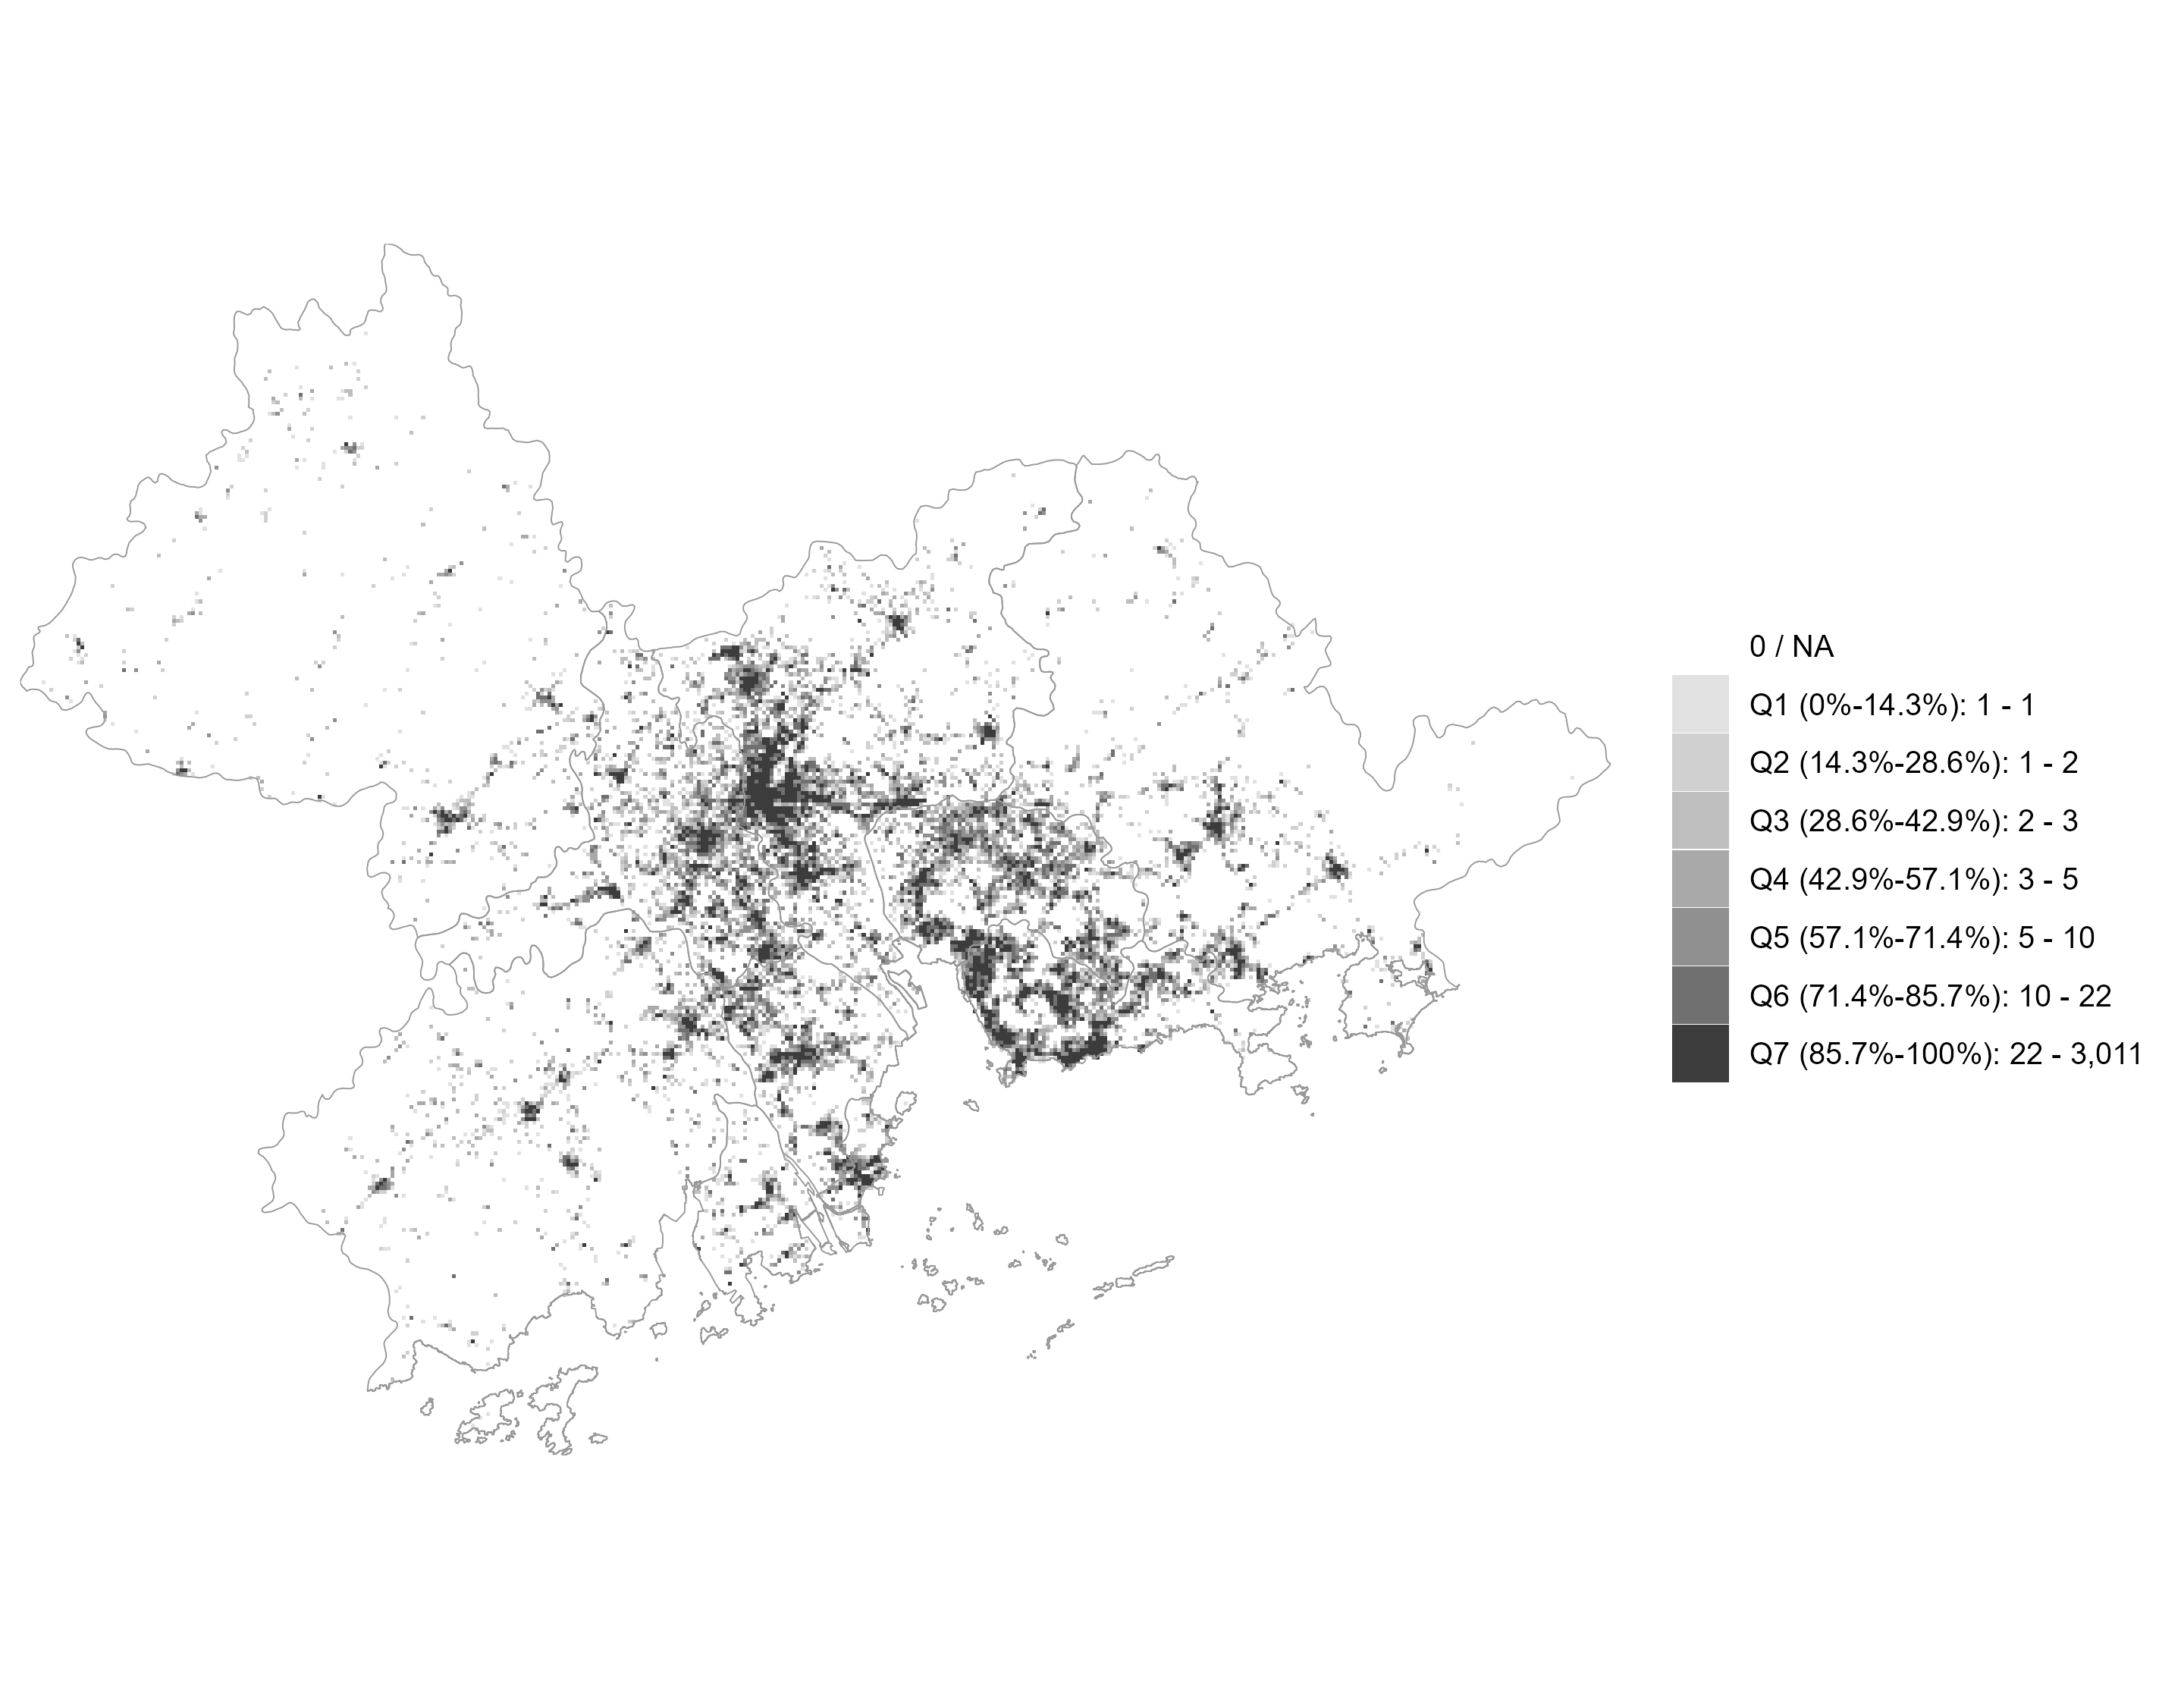
\includegraphics[width=0.95\textwidth]{1.描述性证据/分布图/prd_prefer500m_crime_count_1km.png}
\caption{2015--2020年珠三角犯罪人次分布图}
\label{fig:map_crime}
\end{figure}

本文引入2015--2020年WorldPop项目发布的100m人口栅格数据集，以在计数模型中刻画人口规模差异并将犯罪事件数转换为可比的犯罪强度度量\citep{tatem2017worldpop}。该数据以“每像素居住人口数”为单位，覆盖年度层面的空间人口分布。本文将年度人口栅格与100m主网格对齐，并在半年度面板中沿用对应年份的人口值。考虑到部分网格人口接近0会导致对数偏移项不稳定，本文在构建面板时剔除人口小于1的网格观测；在PPML估计中将$\ln(Pop_{g,t})$作为offset项纳入模型设定（见第 \ref{sec:method_ppml} 节）。人口空间分布示意见附录图 \ref{fig:map_pop}。

\subsection{基于深度学习的城中村网格识别}
本文采用2018年珠三角城中村分布100米栅格数据。具体而言，该数据来自Wu等\citeyearpar{wu2025uvframework}基于Sentinel-2多时相观测与深度学习识别得到的珠江三角洲九市城中村识别结果。该识别结果以100米栅格形式发布，每个栅格的数值表示该栅格内城中村面积占比。\footnote{作为参考，Wu等\citeyearpar{wu2025uvframework}报告其模型在广州—深圳样本训练并外推至珠三角的实验中取得83.33\%的mIoU，较基准方法提升0.46--12.49个百分点。mIoU（平均交并比）是衡量图像分割模型性能的常用指标，取值在0到1之间，值越高代表模型在各个类别上的平均分割效果越好。}本文将城中村面积占比大于0的栅格定义为城中村网格，等于0的栅格定义为非城中村网格。相较传统实地调查或人工矢量化，这类产品在跨城市尺度上具有更强的一致性与可扩展性，能够与本文构建的网格级犯罪面板直接对齐。

本文在基准设定中以100米网格作为空间汇总单位，并在稳健性检验中进一步使用200米、500米等更粗尺度。选择100米主要是为了与城中村识别结果、人口栅格及后续空间融合等数据源保持一致，并在空间细节与样本稀疏性之间取得折中。为便于直观理解，附录图 \ref{fig:uv_scale} 给出城中村空间形态与基准网格尺度的示意。图中红色色块为城中村栅格，颜色越深表示网格中城中村面积占比越接近100\%，颜色越浅则越接近0。本文将所有城中村面积占比大于0的网格定义为城中村网格。



\begin{figure}[H]
\centering
\includegraphics[width=\textwidth]{1.描述性证据/分布图/urban_shape.png}
\caption{珠三角城中村与城区边界分布图}
\label{fig:map_uv}
\end{figure}

本文进一步引入2015年城区范围边界数据，以区分城市核心区与城市边缘区域的城中村。根据\textcite{wanghao2023builtup}给出的2015年城区范围定义，城区范围是指各地级市下辖各区政府所在的连片建成区。相较于通常意义上的“建成区”，这一口径剔除了城市外围孤立分布的建成区斑块，从而更贴近“中心—外围”的空间结构划分。本文使用基于优于2m分辨率地表覆盖数据并结合道路、水系等专题信息自动提取的2015年中国地级以上城市城区范围产品\citep{wanghao2023builtup}，据此将城中村网格划分为城区内与城区外两类，用于后续异质性分析。图 \ref{fig:map_uv} 进一步展示了珠三角范围内城中村网格与城区范围边界的空间分布。图中黄色细线为城区范围边界，红色为城中村网格。

\subsection{县级关税暴露度}
美国2018年三批对华加征关税清单依次为：List 1于2018年7月6日生效，针对约340亿美元商品加征25\%关税；List 2于2018年8月23日生效，针对约160亿美元商品加征25\%关税；List 3于2018年9月24日生效，针对约2000亿美元商品加征10\%关税并在2019年9月上调至25\%。至2018年9月，美国对华平均关税由贸易战前约3.1\%上升至约12.0\%，新增关税覆盖双边贸易的近一半\citep{bown2021trade}。鉴于冲击启动时点集中在2018年下半年，本文在基准设定中将政策冲击时点定义为2018H2。


本文使用2016年中国海关数据集\footnote{中国海关企业层面贸易交易数据可得年份为2000--2016年，取事前最近可得年份。包含企业—产品—目的地维度的进出口额与HS编码信息。通过与工商企业注册信息数据库匹配可以得到企业地理坐标信息，进而确定出口记录归属地。}计算各县（区）对美出口篮子。为了构造县级关税暴露度，本文进一步将出口品类与美国HTSUS编码进行匹配。\footnote{本文采用“先细后粗”的编码匹配策略。中国海关数据的HS编码以6位为核心（8位通常以00结尾，前6位有效），与美国HTSUS编码在前6位上具有可比性，但同一HS-6可能对应多个更细的HTSUS-8子目。本文首先尝试将以00结尾的8位中国海关编码与8位HTSUS编码直接匹配；对剩余部分再按前6位进行匹配。按照该规则，本文在2016年珠三角九市对美出口样本中，首先直接匹配得到21,985条记录；在此基础上再以前6位进行匹配得到40,390条记录；仍有32,254条记录无法匹配到关税清单中的HTSUS编码，可视为未被List 1--3覆盖。}考虑到2018年下半年List 1与List 2税率均为25\%，且List 3在后续上调至25\%，对于匹配到一个或多个List中产品的HS-6产品，本文将其关税税率增量设定为25\%，未匹配产品设定为0\%。附录表 \ref{tab:tariff_match} 汇总了匹配结果与样本规模。

参考贸易冲击文献的暴露度构造思路\citep{amiti2019impact}，本文以2016年县级对美出口结构为初始份额，以产品层面的额外关税变动为外部冲击，构造县级\footnote{珠三角的东莞市与中山市因历史行政体制原因不设县级行政区，市直接管辖镇街。若在市级口径计算关税暴露度，则在本文基准回归加入城市$\times$半年度固定效应后，处理强度将被完全吸收，从而无法识别效应。本文对东莞与中山按初级人民法院的司法辖区分配虚拟的县级行政区划，并分别计算各司法辖区的出口冲击（县级暴露度）。(以镇街为基础单元，东莞包括第一、第二、第三初级人民法院三个司法辖区，中山包括第一、第二初级人民法院两个司法辖区。)}关税暴露度指标：
\begin{equation}
TariffExposure_{c,2018} = \sum_{i} \frac{Export_{c,i,2016}}{TotalExport_{c,2016}} \times \Delta \tau_{i,2018}
\end{equation}
其中，$Export_{c,i,2016}/TotalExport_{c,2016}$表示县（区）$c$在2016年对美国出口中第$i$类产品的份额，$\Delta \tau_{i,2018}$表示2018年关税清单对第$i$类产品施加的额外关税（基准设定下，清单覆盖产品取25\%，其余取0\%）。图 \ref{fig:map_tariff} 展示了该暴露度指标在珠三角内部的空间差异。

\begin{figure}[H]
\centering
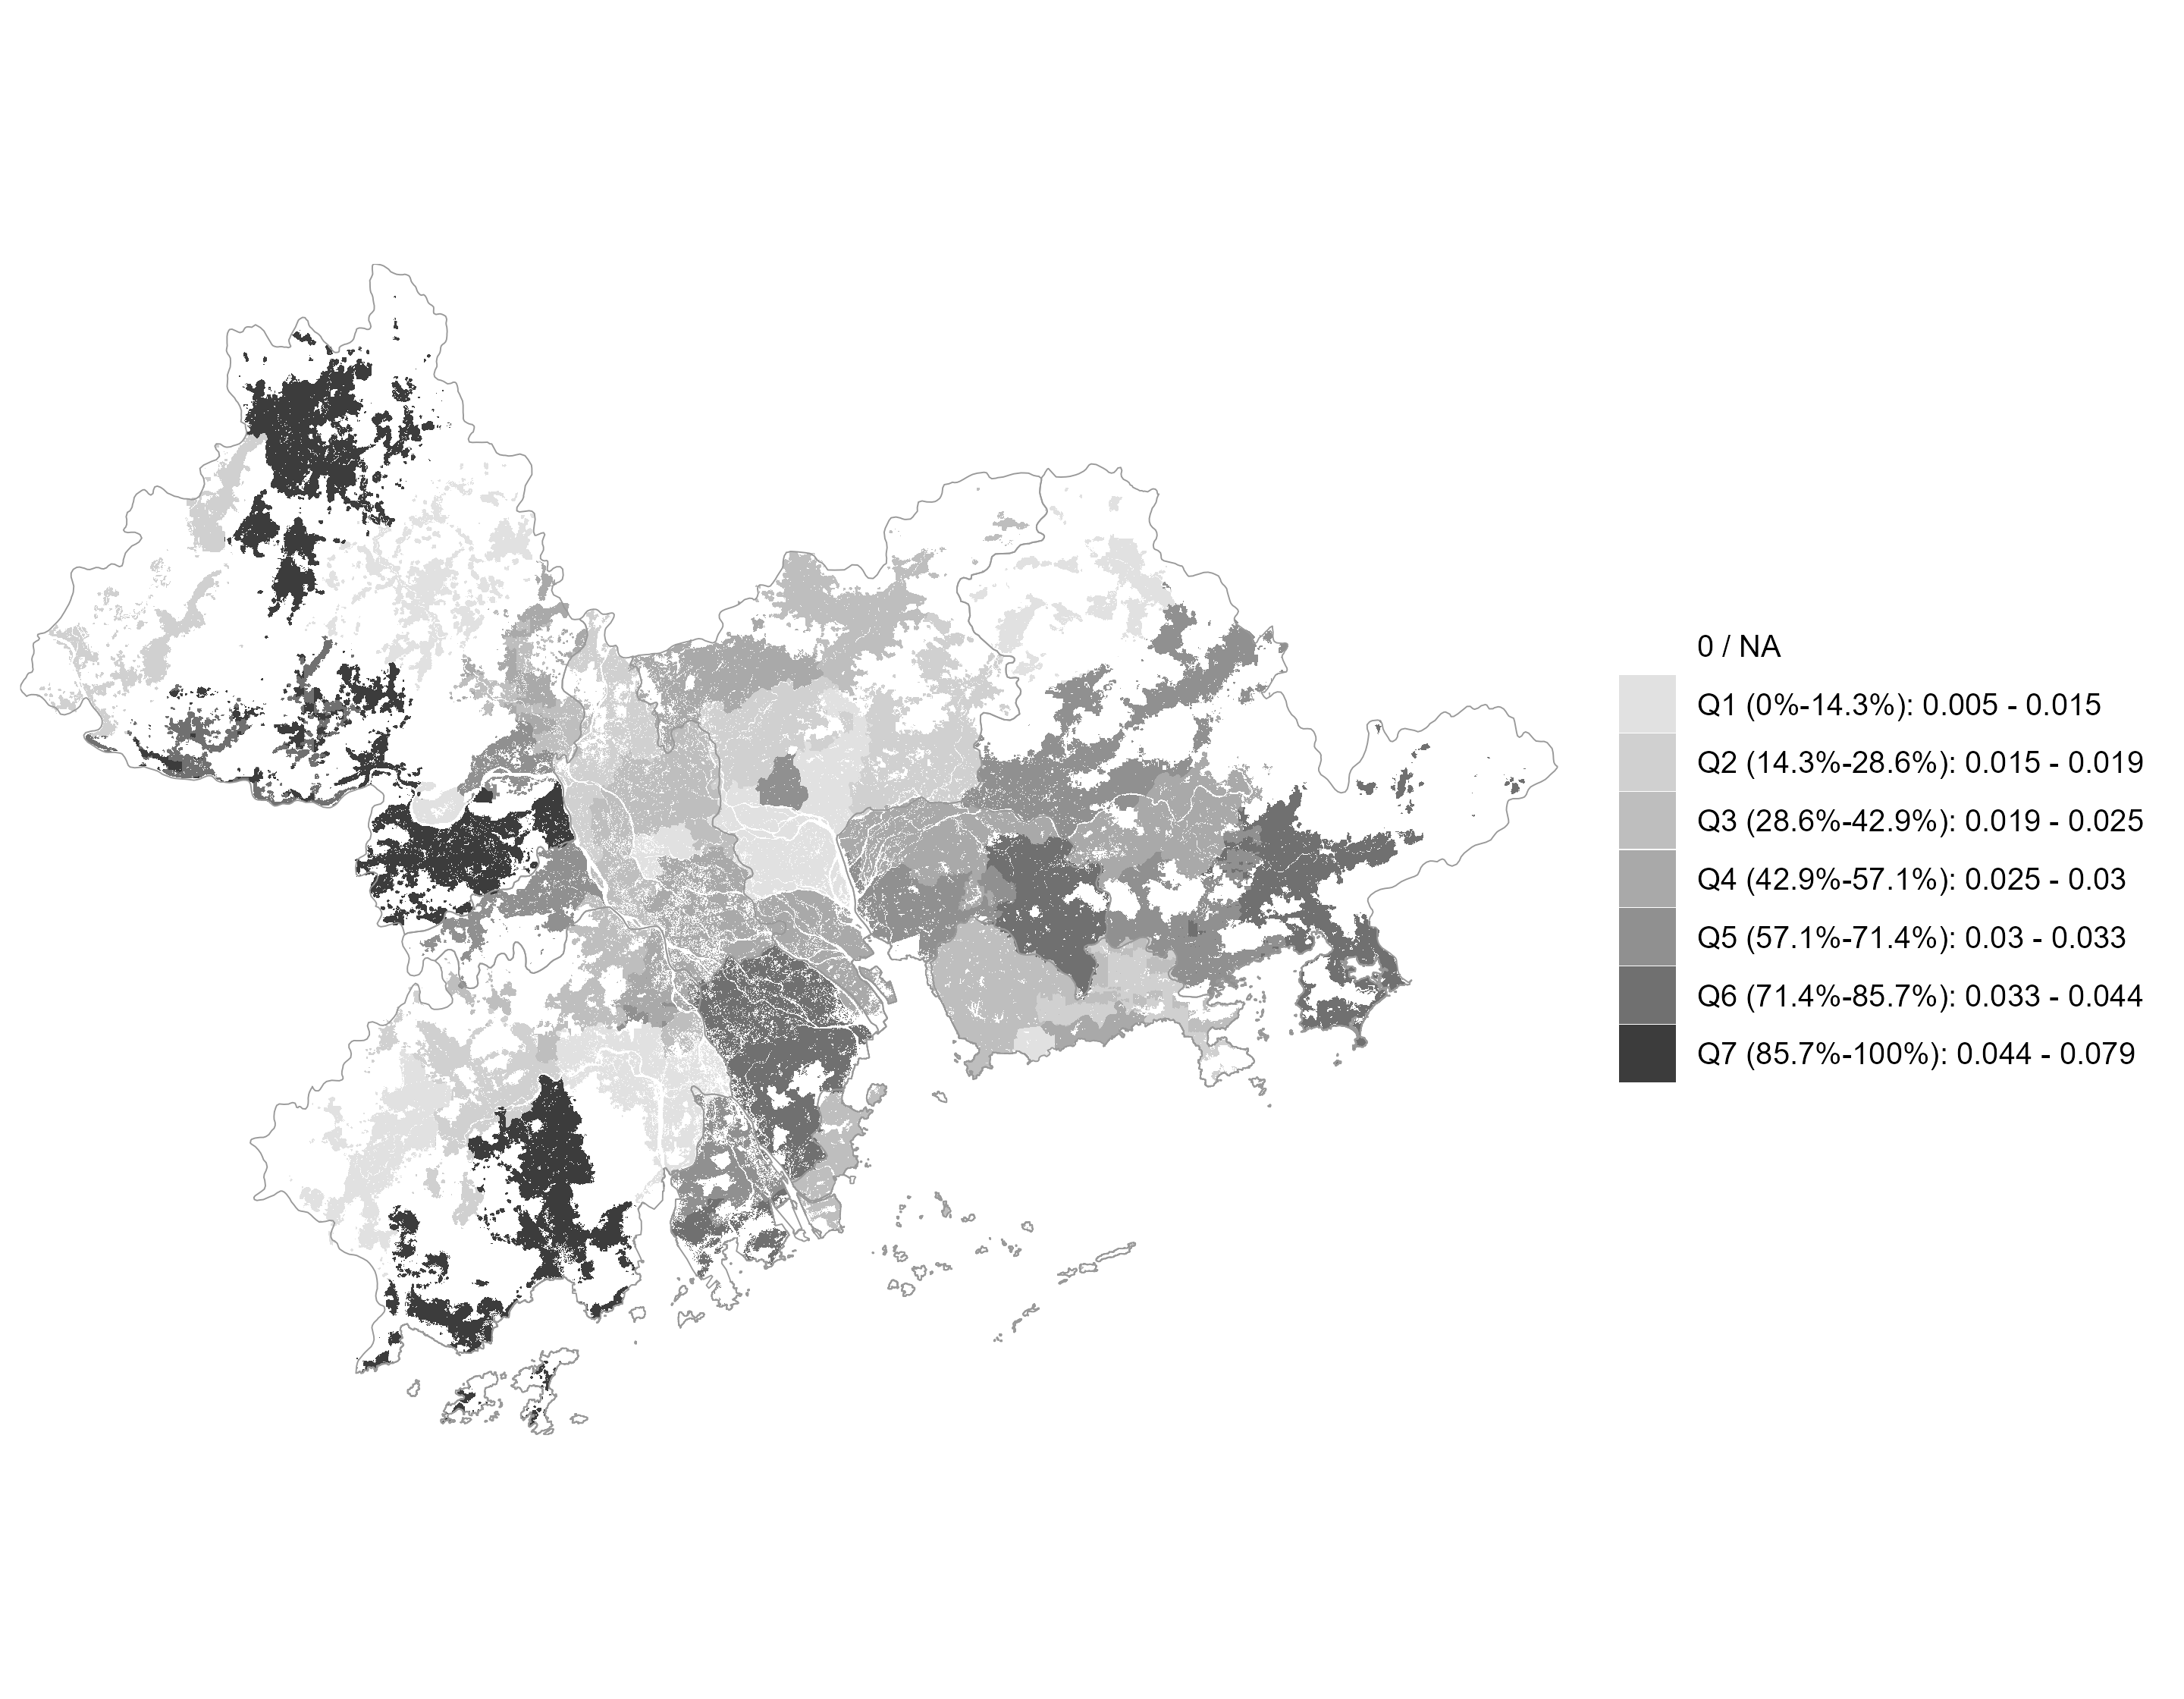
\includegraphics[width=0.95\textwidth]{1.描述性证据/分布图/prd_prefer500m_us_tariff_exposure_4.png}
\caption{2018年珠三角对美出口关税暴露度分布图}
\label{fig:map_tariff}
\end{figure}

除关税暴露度外，本文还为补充分析构造了社会网络、基础设施可达性和住房市场等城中村特征变量。考虑到这些变量与本文的主要结论欠相关，其详细定义、构造过程与示意图移入附录“城中村特征变量说明”部分。

\section{数据描述}
本节对政策实施前样本的基准特征作简要说明。为与后文主线一致，本文将研究对象划分为三类：城区内且城中村面积占比大于0的网格定义为城区内城中村，城区范围外且城中村面积占比大于0的网格定义为城市外围城中村，城区范围内且城中村面积占比等于0的网格定义为正规街区。表 \ref{tab:baseline_main} 报告三类样本的主要基线统计量；完整版本仍保留在附录表 \ref{tab:baseline}。

\begin{table}[H]
\centering
\caption{描述性统计结果}
\label{tab:baseline_main}
\zihao{5}
\begin{adjustbox}{width=\textwidth,center}
\begin{tabular}{lccccc}
\toprule
变量 & 全样本 & 正规街区 & 城中村 & 中心城中村 & 外围城中村 \\
\midrule
关税暴露度 & \makecell{0.029\\(0.016)} & \makecell{0.024\\(0.008)} & \makecell{0.025\\(0.010)} & \makecell{0.025\\(0.008)} & \makecell{0.027\\(0.012)} \\
人口密度 & \makecell{19.102\\(50.674)} & \makecell{54.356\\(94.380)} & \makecell{59.189\\(79.283)} & \makecell{72.760\\(90.596)} & \makecell{35.393\\(45.023)} \\
十万人犯罪率 & \makecell{15.782\\(1520.161)} & \makecell{30.401\\(1999.833)} & \makecell{59.259\\(2695.463)} & \makecell{59.130\\(1358.386)} & \makecell{59.486\\(4094.982)} \\
到公交车站距离 & \makecell{21854.506\\(25800.034)} & \makecell{5198.428\\(4806.057)} & \makecell{7134.018\\(7176.148)} & \makecell{5625.248\\(5146.584)} & \makecell{9779.328\\(9184.640)} \\
到小学距离 & \makecell{1897.568\\(1709.585)} & \makecell{1201.118\\(774.719)} & \makecell{811.575\\(654.294)} & \makecell{723.624\\(559.138)} & \makecell{965.778\\(770.198)} \\
到三甲医院距离 & \makecell{11049.707\\(10904.109)} & \makecell{3440.906\\(2202.143)} & \makecell{4193.076\\(4546.859)} & \makecell{2985.484\\(2118.458)} & \makecell{6310.334\\(6481.760)} \\
到股份制商业银行距离 & \makecell{18566.608\\(24166.442)} & \makecell{2909.621\\(2315.000)} & \makecell{4196.608\\(5095.410)} & \makecell{2482.858\\(2078.694)} & \makecell{7201.306\\(7052.006)} \\
网格数 & 2741736 & 487216 & 156741 & 99823 & 56918 \\
样本期数 & 12 & 12 & 12 & 12 & 12 \\
\bottomrule
\end{tabular}
\end{adjustbox}
\vspace{0.2cm}

\par\raggedright\zihao{5} 注：表中报告各变量的均值，括号内为标准差。
\end{table}

从基准特征看，三类空间单元在对美出口关税暴露度上的差异并不大，这有助于说明后文识别并不是建立在某类空间单元在政策前就具有系统性更高关税暴露度的基础上。相较之下，人口密度、犯罪基准水平和基础设施可达性在城市内部的差异更为明显。城区内城中村的人口规模和公共服务可达性通常优于外围城中村，而外围城中村在交通可达性和夜间灯光等方面更弱，呈现出更典型的城市边缘特征。

另一个重要事实是，城中村尤其是外围城中村在政策前已经具有更高的平均犯罪水平。这意味着后文识别不能依赖横截面均值比较，而必须依赖外生关税冲击带来的差异化变化，并通过固定效应框架尽可能剥离不随时间变化的空间异质性。也正因为如此，本文关注的重点不是“哪里犯罪本来就更多”，而是“冲击之后哪里的犯罪增量更集中”。

\section{实证方法}
\label{sec:method_ppml}
本文采用连续双重差分模型，并以泊松伪极大似然（PPML）方法进行估计。设$Crime_{g,c,t}$表示网格$g$在县（区）$c$、半年度$t$的犯罪事件数，$Exposure_c$为县（区）层面的对美出口关税暴露度，$Post_t$为2018H2及之后的政策后期指示变量。为便于跨地区比较与解释，本文将$Exposure_c$进行标准化处理（均值为0、标准差为1）。为控制人口规模差异并将“事件数”转化为可比的犯罪强度，本文在PPML中加入offset项$\ln(Pop_{g,t})$。基准模型写为：
\begin{equation}
\begin{split}
\mathbb{E}\left[Crime_{g,c,t}\mid X\right]
&=\exp\Big(\beta\cdot Post_t\times Exposure_c+\delta_g+\gamma_{city,t}+\ln(Pop_{g,t})\Big),
\end{split}
\end{equation}
其中，$\delta_g$为网格固定效应，用以吸收不随时间变化的空间异质性；$\gamma_{city,t}$为城市$\times$半年度固定效应，用以控制宏观共振冲击与城市层面的共同趋势。等价地，$\mathbb{E}[Crime_{g,c,t}\mid X]/Pop_{g,t}$服从对数线性指数形式，因此$\beta$识别的是作为比率意义上的处理效应。

选择PPML的关键理由在于：犯罪数据为非负整数计数形式，且在细网格层面零值占比较高，采用对数线性模型会面临$\ln(0)$问题并可能引入选择性样本偏误。PPML能够在不对因变量取对数的情况下直接处理零值，并在条件均值设定正确时作为准极大似然估计量保持一致性；同时该估计对异方差较为稳健，因此常用于估计计数型因变量与引力方程模型\citep{santosSilva2006ppml}。在这类框架下，系数$\beta$可解释为：在其他条件不变时，政策实施期间关税暴露度提高1个标准差，将使条件期望犯罪事件数按$\exp(\beta)-1$的比例变化；当$\beta$较小时，近似为$\beta\times100\%$的百分比变化。标准误均按县（区）层面进行聚类，以允许同一县（区）内部存在任意形式的序列相关与空间相关。上述连续双重差分模型的有效性建立在平行趋势假设之上，即在2018年关税冲击前，不同关税暴露度地区的城中村与正规街区犯罪率演变趋势并不存在系统性分化。本文将在后续实证中通过事件研究对此假设进行检验。

\chapter{实证分析}

\section{基准结果}
表 \ref{tab:main_100m} 报告了本文的基准回归结果，表明关税冲击主要表现为城中村犯罪上升：当关税暴露度提高1个标准差时，城中村网格犯罪强度上升约20.6\%，且在1\%水平显著；相比之下，正规街区和全样本的对应估计均不显著。这一结果说明，关税冲击的治安后果并不是城市范围内的平均上升，而是首先集中出现在特定微观空间单元。

\begin{table}[H]
\centering
\caption{基准回归结果}
\label{tab:main_100m}
\zihao{5}
\begin{tabular*}{\textwidth}{@{\extracolsep{\fill}}lccc}
\toprule
 & 全样本 & 正规街区 & 城中村 \\
\midrule
$Post\times Exposure$ & 0.046 & 0.110 & 0.188*** \\
 & (0.070) & (0.116) & (0.070) \\
\midrule
样本量 & 32,900,832 & 7,044,024 & 1,880,892 \\
Pseudo $R^2$ & 0.177 & 0.078 & 0.070 \\
\bottomrule
\end{tabular*}
\vspace{0.2cm}

\par\raggedright\zihao{5} 注：括号内为按县（区）聚类标准误。* $p<0.10$，** $p<0.05$，*** $p<0.01$。回归设定为PPML连续DID，因变量为网格半年度犯罪事件数，使用$\ln(Pop_{g,t})$作为offset，并控制县（区）固定效应与城市$\times$半年度固定效应。后续表格若无特殊说明，回归规格均与本表一致。
\end{table}

为进一步刻画动态路径并检验事前平行趋势，图 \ref{fig:event_uv} 给出了城中村样本的事件研究结果。政策前各期系数未显示出系统性的差异趋势，而政策实施后系数明显上升，支持本文的识别设定并表明冲击后城中村犯罪存在持续一段时期的抬升。

\begin{figure}[H]
\centering
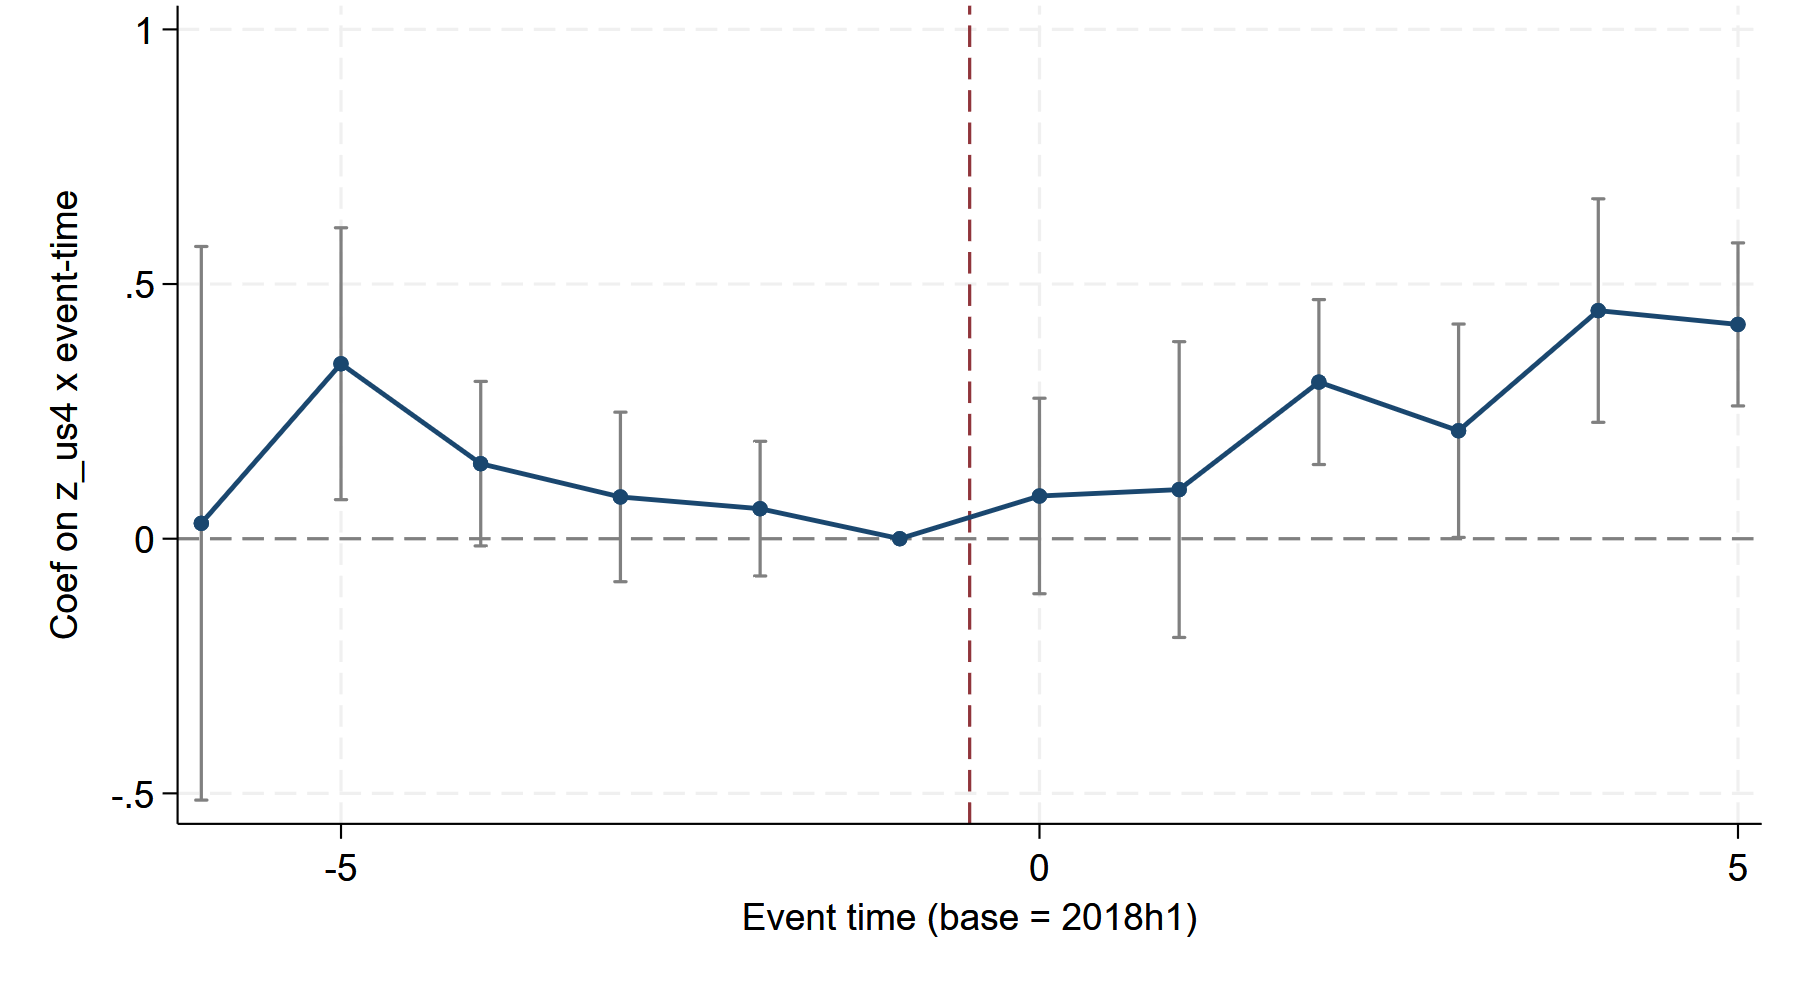
\includegraphics[width=0.9\textwidth]{event_uv_countyfe_100m_v10.png}
\caption{事件研究图}
\label{fig:event_uv}
\end{figure}

\section{城市内部异质性}
若只停留在“城中村与非城中村”的比较，仍不足以说明城市内部冲击承载的具体落点。表 \ref{tab:hetero_core_peri} 进一步区分正规街区、城区内城中村和城市外围城中村。结果显示，外围城中村的估计值为0.1583，在1\%水平显著；城区内城中村估计值为0.1769，但仅边际显著；正规街区不显著。换言之，冲击的犯罪影响主要集中体现在城市外围城中村，这也是本研究主要的经验事实。外围城中村通常具有更弱的正式就业连接、更远的交通与公共服务距离，以及与郊区制造业就业更紧密的联系，因此更容易在外部需求收缩时呈现更强的犯罪响应。相比之下，城区内城中村虽然也存在一定的犯罪响应，但其显著性较弱且不够稳定，这可能与其更好的公共服务可达性、更强的社会网络以及更多的非制造业就业机会有关，从而在一定程度上缓冲了冲击带来的治安风险。正规街区则没有显示出明显的犯罪响应，进一步支持了冲击效应在城市内部具有明显的空间集中性。

\begin{table}[H]
\centering
\caption{空间位置异质性}
\label{tab:hetero_core_peri}
\zihao{5}
\begin{tabular*}{\textwidth}{@{\extracolsep{\fill}}lccc}
\toprule
 & 正规街区 & 中心城中村 & 外围城中村 \\
\midrule
$Post\times Exposure$ & 0.093 & 0.177+ & 0.158*** \\
 & (0.128) & (0.122) & (0.058) \\
\midrule
样本量 & 5,846,172 & 1,197,852 & 674,743 \\
Pseudo $R^2$ & 0.086 & 0.055 & 0.096 \\
\bottomrule
\end{tabular*}
\vspace{0.2cm}

\par\raggedright\zihao{5} 注：样本为100m网格。$+$表示$p<0.15$；* $p<0.10$，** $p<0.05$，*** $p<0.01$。
\end{table}



\section{分案由的进一步讨论}
表 4 和表 5 进一步表明，关税冲击对城中村犯罪的影响并不是由某一单一案由驱动，而是具有较为清晰的案由结构差异。首先从四类案由大类看，财产型、冲动型、企业型和地下经济类犯罪在城中村样本中的系数均为正，其中冲动型犯罪、企业犯罪和地下经济犯罪的估计值相对更大；相比之下，正规街区样本的对应估计普遍不显著。这说明关税冲击带来的治安风险主要集中在城中村内部，并且这种风险具有较广泛的犯罪类型覆盖。

\begin{table}[H]
\centering
\caption{案由大类的进一步讨论}
\label{tab:hetero_4cat}
\zihao{5}
\begin{tabular*}{\textwidth}{@{\extracolsep{\fill}}lcccc}
\toprule
案由大类 & 正规街区 & 城中村 & 中心城中村 & 外围城中村 \\
\midrule
财产型犯罪 & \makecell{0.101\\(0.150)} & \makecell{0.190**\\(0.090)} & \makecell{0.122\\(0.172)} & \makecell{0.190***\\(0.062)} \\
冲动型犯罪 & \makecell{0.075\\(0.209)} & \makecell{0.320***\\(0.101)} & \makecell{0.344\\(0.247)} & \makecell{0.292***\\(0.061)} \\
企业犯罪 & \makecell{0.186+\\(0.125)} & \makecell{0.422**\\(0.184)} & \makecell{0.497+\\(0.331)} & \makecell{0.507**\\(0.246)} \\
地下经济犯罪 & \makecell{0.136\\(0.141)} & \makecell{0.178***\\(0.069)} & \makecell{0.104\\(0.209)} & \makecell{0.201***\\(0.049)} \\
\bottomrule
\end{tabular*}
\vspace{0.15cm}

\par\raggedright\zihao{5} 注：表中为$Post\times Exposure$的系数，+ $p<0.15$，* $p<0.10$，** $p<0.05$，*** $p<0.01$。
\end{table}

进一步结合表 4 的城区内外分组结果可以看到，外围城中村上的案由响应更为清晰。财产型犯罪和地下经济犯罪在外围城中村上均显著为正，冲动型犯罪和企业犯罪的估计值也明显高于正规街区，这说明城市外围城中村不仅是总犯罪上升的主要承载空间，在分类型犯罪上也更容易集中体现冲击效应。相较之下，城区内城中村虽然若干系数也为正，但显著性和稳定性明显弱于外围城中村。

将案由进一步细分到16类后，首先从城中村整体来看，财产型犯罪中的盗窃、诈骗、敲诈勒索显著增加，公共安全、暴力、交通犯罪三种冲动型犯罪也均显著增加，这表明由于贸易冲击导致的经济压力和失业风险，激发了以获取经济利益为直接目的的犯罪以及多与心理压力关联的冲动型社会事件。企业犯罪中知识产权犯罪显著增加，贿赂在15\%水平显著，表明企业在面临外需下行和关税冲击时可能更多地利用涉嫌侵权的低成本途径维持生产或通过贿赂等灰色手段谋求生存空间。地下经济犯罪中，毒品犯罪显著增加，表明宏观冲击可能促使部分边缘与弱势人群转向非法获利的微观地下网络。相比而言，正规街区仅敲诈勒索在15\%水平边缘显著增加，且系数较小，表明正规街区受因波动引发的直接治安影响较小；此外走私犯罪在正规街区显著增加，显示了正规国际贸易途径的壁垒可能导致非正规途径贸易增加。进一步考察城中村内部异质性，大部分案由（如诈骗、暴力、毒品）在外围城中村表现出比在中心城中村和城中村全体中更强的显著性和响应幅度。值得注意的是，交通犯罪和淫秽相关犯罪在中心城中村网格的显著性高于外围城中村，这可能与内城城中村拥有更高密度的微观交通以及更集中的人员服务流动有关。此外，抢劫犯罪在外围城中村显著增加，这一案由结果在整体看待城中村时并不显著，这表明在面临宏观经济冲击时，边缘外围区域不仅承担了更大的犯罪绝对增量，而且更容易滋生暴力程度较高的恶性财产剥夺犯罪。

\begin{table}[H]
\centering
\caption{16类细分案由的进一步讨论}
\label{tab:hetero_16cat}
\zihao{5}
\begingroup
\setlength{\tabcolsep}{1.2pt}
\renewcommand{\arraystretch}{0.75}
\begin{tabular*}{\textwidth}{@{\extracolsep{\fill}}llcccc}
\toprule
案由大类 & 16类案由 & 正规街区 & 城中村 & 中心城中村 & 外围城中村 \\
\midrule
\multirow{4}{*}{财产型犯罪} & 盗窃 & \makecell{0.117\\(0.152)} & \makecell{0.163*\\(0.086)} & \makecell{0.183\\(0.181)} & \makecell{0.120**\\(0.058)} \\
 & 诈骗 & \makecell{-0.054\\(0.201)} & \makecell{0.548***\\(0.174)} & \makecell{0.516+\\(0.330)} & \makecell{0.464***\\(0.101)} \\
 & 抢劫 & \makecell{0.095\\(0.305)} & \makecell{0.062\\(0.230)} & \makecell{-0.511\\(0.363)} & \makecell{0.454***\\(0.114)} \\
 & 敲诈勒索 & \makecell{0.887+\\(0.569)} & \makecell{0.810*\\(0.418)} & \makecell{-0.420\\(0.912)} & \makecell{6.204\\(4.320)} \\
\midrule
\multirow{3}{*}{冲动型犯罪} & 公共安全 & \makecell{0.637\\(0.495)} & \makecell{1.120***\\(0.355)} & \makecell{0.464\\(0.725)} & \makecell{1.866**\\(0.762)} \\
 & 暴力 & \makecell{0.155\\(0.212)} & \makecell{0.312***\\(0.112)} & \makecell{0.317\\(0.272)} & \makecell{0.298***\\(0.067)} \\
 & 交通犯罪 & \makecell{-0.260\\(0.372)} & \makecell{0.272**\\(0.130)} & \makecell{0.833*\\(0.434)} & \makecell{0.134+\\(0.093)} \\
\midrule
\multirow{4}{*}{企业犯罪} & 知识产权 & \makecell{0.018\\(0.173)} & \makecell{0.464**\\(0.223)} & \makecell{0.481\\(0.431)} & \makecell{0.782*\\(0.457)} \\
 & 制假售假 & \makecell{0.417\\(0.435)} & \makecell{0.147\\(0.627)} & \makecell{0.157\\(0.599)} & \makecell{3.769\\(11.572)} \\
 & 贿赂 & \makecell{-0.082\\(0.230)} & \makecell{2.084+\\(1.369)} & \makecell{1.811\\(1.539)} & \makecell{0.626\\(0.700)} \\
 & 金融 & \makecell{-0.011\\(0.430)} & \makecell{-0.416\\(0.659)} & \makecell{-0.285\\(0.981)} & \makecell{--\\(--)} \\
\midrule
\multirow{5}{*}{地下经济犯罪} & 毒品 & \makecell{0.098\\(0.146)} & \makecell{0.183**\\(0.087)} & \makecell{-0.031\\(0.270)} & \makecell{0.196***\\(0.063)} \\
 & 赌博 & \makecell{0.093\\(0.172)} & \makecell{0.085\\(0.151)} & \makecell{0.035\\(0.307)} & \makecell{0.179\\(0.129)} \\
 & 淫秽 & \makecell{0.186\\(0.356)} & \makecell{0.188\\(0.167)} & \makecell{0.222+\\(0.153)} & \makecell{0.191\\(1.261)} \\
 & 走私 & \makecell{1.123***\\(0.077)} & \makecell{-1.677\\(3.698)} & \makecell{-1.759\\(4.441)} & \makecell{--\\(--)} \\
 & 非法迁徙 & \makecell{-0.134\\(0.579)} & \makecell{--\\(--)} & \makecell{--\\(--)} & \makecell{--\\(--)} \\
\bottomrule
\end{tabular*}
\endgroup
\vspace{0.15cm}

\par\raggedright\zihao{5} 注：表中为$Post\times Exposure$的系数，+ $p<0.15$，* $p<0.10$，** $p<0.05$，*** $p<0.01$；“--”表示该子样本该案由无法估计或样本不足。
\end{table}



进一步从犯罪人画像看，关税冲击带来的犯罪增加更多体现在男性、有业和低教育群体上。这些结果并不意味着“特定人群本身更危险”，而是表明冲击后的司法可观测犯罪结构具有明显差异。由于裁判文书记录口径与案件进入司法程序的选择性都会影响样本呈现，本文将其作为对风险承载结构的描述，而非强因果机制识别。

\begin{table}[H]
\centering
\caption{被告人身份异质性}
\label{tab:hetero_defendant}
\zihao{5}
\begin{adjustbox}{width=\textwidth}
\begin{tabular}{lcccccccc}
\toprule
 & \multicolumn{2}{c}{就业状态} & \multicolumn{2}{c}{性别} & \multicolumn{2}{c}{民族} & \multicolumn{2}{c}{教育} \\
\cmidrule(lr){2-3}\cmidrule(lr){4-5}\cmidrule(lr){6-7}\cmidrule(lr){8-9}
案由类别 & 有业 & 无业 & 男性 & 女性 & 汉族 & 少数民族 & 高教育 & 低教育 \\
\midrule
总犯罪 & \makecell{0.152***\\{[0.036]}} & \makecell{-0.126\\{[0.219]}} & \makecell{0.124***\\{[0.040]}} & \makecell{0.025\\{[0.166]}} & \makecell{0.132***\\{[0.039]}} & \makecell{0.012\\{[0.134]}} & \makecell{-0.014\\{[0.105]}} & \makecell{0.138***\\{[0.039]}} \\
财产型 & \makecell{0.087\\{[0.123]}} & \makecell{0.069\\{[0.202]}} & \makecell{-0.077\\{[0.091]}} & \makecell{0.079\\{[0.179]}} & \makecell{-0.682***\\{[0.190]}} & \makecell{0.152\\{[0.172]}} & \makecell{0.129**\\{[0.051]}} & \makecell{-1.051***\\{[0.389]}} \\
冲动型 & \makecell{0.466**\\{[0.211]}} & \makecell{0.041\\{[0.194]}} & \makecell{0.153**\\{[0.063]}} & \makecell{0.165\\{[0.175]}} & \makecell{-0.142\\{[0.134]}} & \makecell{0.175\\{[0.156]}} & \makecell{0.178***\\{[0.061]}} & \makecell{-0.844\\{[0.959]}} \\
企业型 & \makecell{0.513***\\{[0.106]}} & \makecell{-0.135\\{[0.367]}} & \makecell{0.261\\{[0.328]}} & \makecell{-0.160\\{[0.459]}} & \makecell{0.032\\{[0.638]}} & \makecell{-0.101\\{[0.359]}} & \makecell{0.208**\\{[0.099]}} & \makecell{0.706\\{[0.739]}} \\
地下经济 & \makecell{0.000\\{[0.092]}} & \makecell{0.138\\{[0.165]}} & \makecell{-0.035\\{[0.107]}} & \makecell{0.112\\{[0.198]}} & \makecell{-0.641**\\{[0.274]}} & \makecell{0.168\\{[0.140]}} & \makecell{0.104***\\{[0.040]}} & \makecell{-0.423\\{[0.291]}} \\
\bottomrule
\end{tabular}
\end{adjustbox}
\vspace{0.2cm}

\par\raggedright\zihao{5} 注：表中数值为$Post\times Exposure$的系数，* $p<0.10$，** $p<0.05$，*** $p<0.01$。
\end{table}

此外，附录中的相关讨论显示，距离学校、基层医疗和交通站点更近的城中村，在短期内往往出现更强的犯罪响应。这一结果说明，设施更好并非必然缓冲风险，反而更可能暗示了设施密集区域具有更高的人群相遇概率和更活跃的日常活动场景，从而在负向外生冲击下更容易形成短期的治安冲突。与此同时，菜系分布指标和餐馆密度等社会互动结构变量在部分样本中表现出一定程度的缓冲作用，尤其是外围城中村中较高的餐馆密度与较弱的冲动型犯罪响应存在相关性。这些结果更多体现了微观活动场景的相关关联，由于这类变量在实际含义上存在复合性（如可能同时反映同乡网络、包容性或市场活力），本研究将此类发现视为启发性的探讨。

\section{稳健性检验}
稳健性分析主要服务于两个问题：第一，结果是否依赖于关税暴露度的具体构造；第二，结果是否可能由空间上的偶然相关造成。表 \ref{tab:robust_shares} 显示，当将基准设定由“对美出口暴露度且List 3按25\%处理”改为其他口径后，点估计明显减弱，说明本文识别到的效应主要来自贸易战中被明确加征关税的对美出口链条，而非一般性的外需波动。

\begin{table}[H]
\centering
\caption{稳健性 不同暴露度口径与税率设定}
\label{tab:robust_shares}
\zihao{5}
\begin{tabular*}{\textwidth}{@{\extracolsep{\fill}}lccc}
\toprule
 & 基准：对美出口暴露度 & 对美出口暴露度 & 全口径出口暴露度 \\
 & （List3=25\%） & （List3=10\%） & （List3=25\%） \\
\midrule
$Post\times Exposure$ & 0.188*** & 0.116 & 0.032 \\
 & (0.070) & (0.086) & (0.108) \\
\midrule
样本量 & 1,880,892 & 1,880,892 & 1,880,892 \\
\bottomrule
\end{tabular*}
\vspace{0.2cm}

\par\raggedright\zihao{5} 注：样本为100m城中村网格。* $p<0.10$，** $p<0.05$，*** $p<0.01$。
\end{table}

空间随机化结果如图 \ref{fig:spatial_perm} 所示。真实估计值显著偏离随机化分布的中心区域，这意味着主要结果并不容易由纯粹的空间巧合解释。标准误口径与缩尾稳健性的完整结果则移至附录表 \ref{tab:robust_se} 和表 \ref{tab:robust_winsor}。

\begin{figure}[H]
\centering
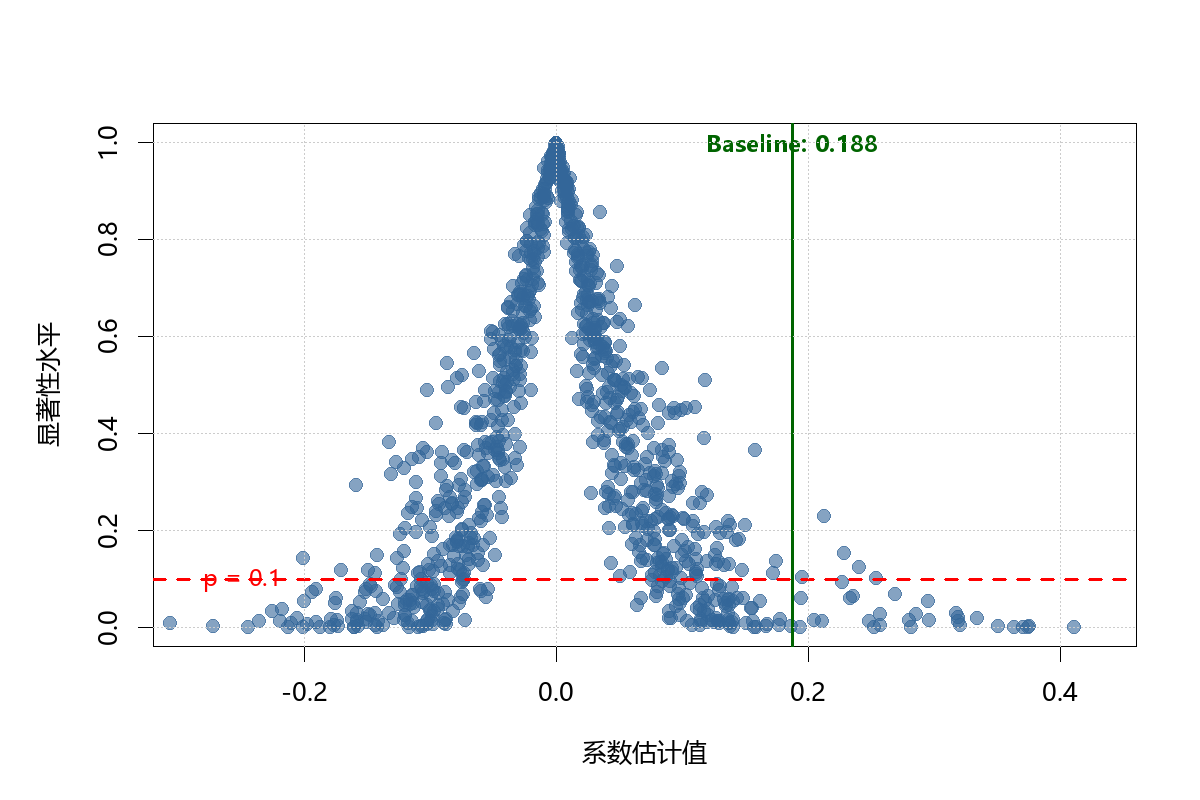
\includegraphics[width=0.9\textwidth]{spatial_permutation_scatter_v1.png}
\caption{空间随机化推断（1,000次） 真实估计与随机化分布对比}
\label{fig:spatial_perm}
\end{figure}
此外，我们还对结果的稳健性进行了多方面检验，包括使用不同的标准误聚类口径（如城市层面聚类）和对极端值进行缩尾处理（见附录表 \ref{tab:robust_se} 和表 \ref{tab:robust_winsor}）。总体来看，主要结论在这些不同设定下仍然保持稳定，进一步增强了本文实证发现的可信度。

\chapter{结论与政策含义}
本文主要考察了宏观国际贸易摩擦向城市微观空间传递的显性社会成本。利用2018年美国对华加征关税这一纯外生冲击，结合县（区）层面的关税暴露度（Shift-share设计）与100米网格层面的半年度犯罪面板，本文评估了关税冲击对珠三角地区城市内部的正规与非正规街区（城中村）犯罪强度的异质性影响。基准与异质性结果表明：关税暴露度每提高一个标准差，城中村网格的犯罪事件显著上升约20.6\%，而正规街区不受明显影响。更为重要的是，这种由外部冲击引起的治安恶化并非被整座整市均匀消化，而是极度不平衡地向区位边缘、发展较弱的外围城中村集中；影响类型则主要表现为财产型、冲动型及地下经济犯罪的激增。

本研究的实证发现对现有文献形成了三点重要补充：第一，本文拓展了关于宏观经济波动与犯罪关系的文献，明确了单边加征关税这一清晰的外生政策所引发的社会后果；第二，突破了以往关于贸易摩擦后果仅停留于企业利润与就业等传统经济指标的局限，揭示了其对城市治理产生的负外部社会成本；第三，本文将大语言模型（LLM）引入微观空间数据构建中，将研究尺度从传统的市、县下沉至100米的基层网格，为宏观经济冲击在城市微观异质性空间上的非均匀分配提供了坚实的量化证据。

政策层面，本文的结果警示，在宏观经济面临外部下行压力或贸易摩擦加剧的时期，城市治理与风险防范应当尽早识别并关注城市内部更具脆弱性的微观空间——特别是位于城市外围的城中村。在具体施策时，治理部门需将有限的治安维护、社区援助与流动人口公共服务资源进行精准配置，针对性地向这些高承压节点倾斜，从而在避免局部社会矛盾集中爆发的同时，提升整座城市的底层韧性。

此外，本研究也存在一定的局限性。首先，受客观条件所限，本研究的犯罪面板数据主要依赖于能够公开获取的刑事裁判文书；尽管利用大语言模型扩展了数据广度，但仍可能遗漏尚未进入司法诉讼环节的轻微治安事件，存在结果滞延与测量误差。其次，本研究立足于珠三角这一外向型经济高度发达且城中村密集的特定区域，其结论推广至非外向主导的内陆城市或其他类型的城市边缘地带时，仍有待考察外部效度。未来若能进一步获取覆盖全案由的微观警情数据，或与个体流动及微观制造业企业经营动态数据相匹配，将有助于深入揭示外源冲击向城市局部空间传导并最终转化为微观犯罪压力的具体机制。


\clearpage
\nocite{yi2023povertycrime,xu2021tariffs}
\printbibliography[heading=bibintoc,title={参考文献}]

\clearpage
\thispagestyle{plain}
{\centering\songti\zihao{4}\bfseries 中央财经大学本科毕业论文（设计）原创性声明\par}
\vspace{2\baselineskip} % 标题与正文间距加一行
\songti\zihao{-4}
本人郑重声明：所提交的毕业论文（设计）《企业营销能力的影响因素探究——基于竞争环境和组织学习的视角》，是本人在指导老师的指导下独立进行研究工作所取得的成果。除文中已经注明引用的内容外，不含任何其他个人或集体已经发表或撰写过的作品成果，不存在购买、由他人代写、剽窃和伪造数据等作假行为。对本文研究/设计做出重要贡献的个人和集体，均已在文中以明确方式标明。本人完全意识到本声明的法律结果，如违反有关规定或上述声明，愿意承担由此产生的一切后果。\par
\vspace{3\baselineskip} % 正文与签名区域增加一行
\noindent\begin{tabular*}{\textwidth}{@{\extracolsep{\fill}}p{0.46\textwidth}p{0.46\textwidth}}
论文作者签名：&签字日期：  \hspace{1em} 年 \hspace{0.5em} 月 \hspace{0.5em} 日
\end{tabular*}

\vspace{4\baselineskip} % 调整两部分间距
{\centering\songti\zihao{4}\bfseries 本科毕业论文（设计）版权使用授权书\par}
\vspace{2\baselineskip} % 标题与正文间距加一行
\songti\zihao{-4}
本人完全了解中央财经大学有权保留并向国家有关部门或机构送交本论文的复印件和磁盘，允许论文被查阅和借阅。本人授权中央财经大学可以将本人的毕业论文（设计）的全部或部分内容编入有关数据库进行检索和传播，可以采用影印、缩印或扫描等复制手段保存、汇编论文。\par
\vspace{3\baselineskip} % 正文与签名区域增加一行
\noindent\begin{tabular*}{\textwidth}{@{\extracolsep{\fill}}p{0.46\textwidth}p{0.46\textwidth}}
论文作者签名：&导师签名：
\end{tabular*}

\vspace{2\baselineskip} % 签名与日期之间增加一行
\noindent\begin{tabular*}{\textwidth}{@{\extracolsep{\fill}}p{0.46\textwidth}p{0.46\textwidth}}
签字日期：  \hspace{1em} 年 \hspace{0.5em} 月 \hspace{0.5em} 日&签字日期：  \hspace{1em}  年 \hspace{0.5em} 月 \hspace{0.5em} 日
\end{tabular*}

\clearpage
\thispagestyle{plain}
\ifdefined\NoAcknowledgements
% (致谢页按需隐藏)
\else
{\centering\songti\zihao{4}\bfseries 致谢\par}
\vspace{1em}
\songti\zihao{-4}
感谢指导教师方明老师在文章选题、实证方面的悉心指导栽培。我常常粗心大意犯错导致需要返工，方老师对我每次失败都非常宽容并给予耐心而切中肯綮的指导。感谢导师路乾老师、中国城市与小城镇改革发展研究中心张慧强老师提供的实地调研机会和方法指导，我从他们身上学到研究真实世界经济问题原来是如此有趣且有价值的事。最后感谢基地和学院提供的平台和栽培，胡志安老师对计量文章严谨与品味的强调，召鹏老师、冬梅院长对学生的提携与关怀都让我受益匪浅，感念终身。与王家乐同学的讨论让我在几次选题调整的过程中不至于思维闭塞，基地的同窗们也总能给我鼓舞。本文选题阶段在基地熊勇杰学长和北大国发院叶濯缨学长组织的经济研究社团进行过汇报，并在参与社团日常讨论的过程中得到许多有益的启发和资源，在此也感谢学长们的组织运营。\par
\fi

\clearpage
\appendix
\chapter*{附录}

\addcontentsline{toc}{chapter}{附录}
\setcounter{table}{0}
\renewcommand{\tablename}{附表}
\renewcommand{\thetable}{\arabic{table}}
\setcounter{figure}{0}
\renewcommand{\figurename}{附图}
\renewcommand{\thefigure}{\arabic{figure}}

\section{数据与变量附表}
\begin{table}[H]
\centering
\caption{案由大类与16类案由及样本分布}
\label{tab:crime_categories}
\zihao{5}
\begin{adjustbox}{width=\textwidth}
\begin{tabular}{p{3.0cm} p{8.8cm} r}
\toprule
案由大类（母分类） & 16类案由（子分类） & 数量 \\
\midrule
\multicolumn{3}{l}{\textbf{财产型犯罪}} \\
 & 盗窃（Stealing） & 47,200 \\
 & 抢劫（Robbery） & 6,285 \\
 & 诈骗（Fraud/Defraud） & 7,913 \\
 & 敲诈勒索（Extortion） & 1,160 \\
\midrule
\multicolumn{3}{l}{\textbf{冲动型犯罪}} \\
 & 暴力（Violent crimes） & 25,820 \\
 & 公共安全（Public security） & 2,327 \\
 & 交通犯罪（Traffic felony） & 11,131 \\
\midrule
\multicolumn{3}{l}{\textbf{企业犯罪}} \\
 & 贿赂（Bribery） & 1,576 \\
 & 金融（Finance） & 1,734 \\
 & 制假售假（Counterfeiting） & 1,306 \\
 & 知识产权（IP infringement） & 7,651 \\
\midrule
\multicolumn{3}{l}{\textbf{地下经济犯罪}} \\
 & 毒品（Drugs） & 25,744 \\
 & 赌博（Gambling） & 12,321 \\
 & 淫秽（Prostitution） & 4,098 \\
 & 走私（Smuggling） & 946 \\
 & 非法迁徙（Migration） & 1,129 \\
\midrule
\multicolumn{3}{l}{\textbf{其他}} \\
 & 其他 & 819 \\
\bottomrule
\end{tabular}
\end{adjustbox}
\end{table}

\begin{figure}[H]
\centering
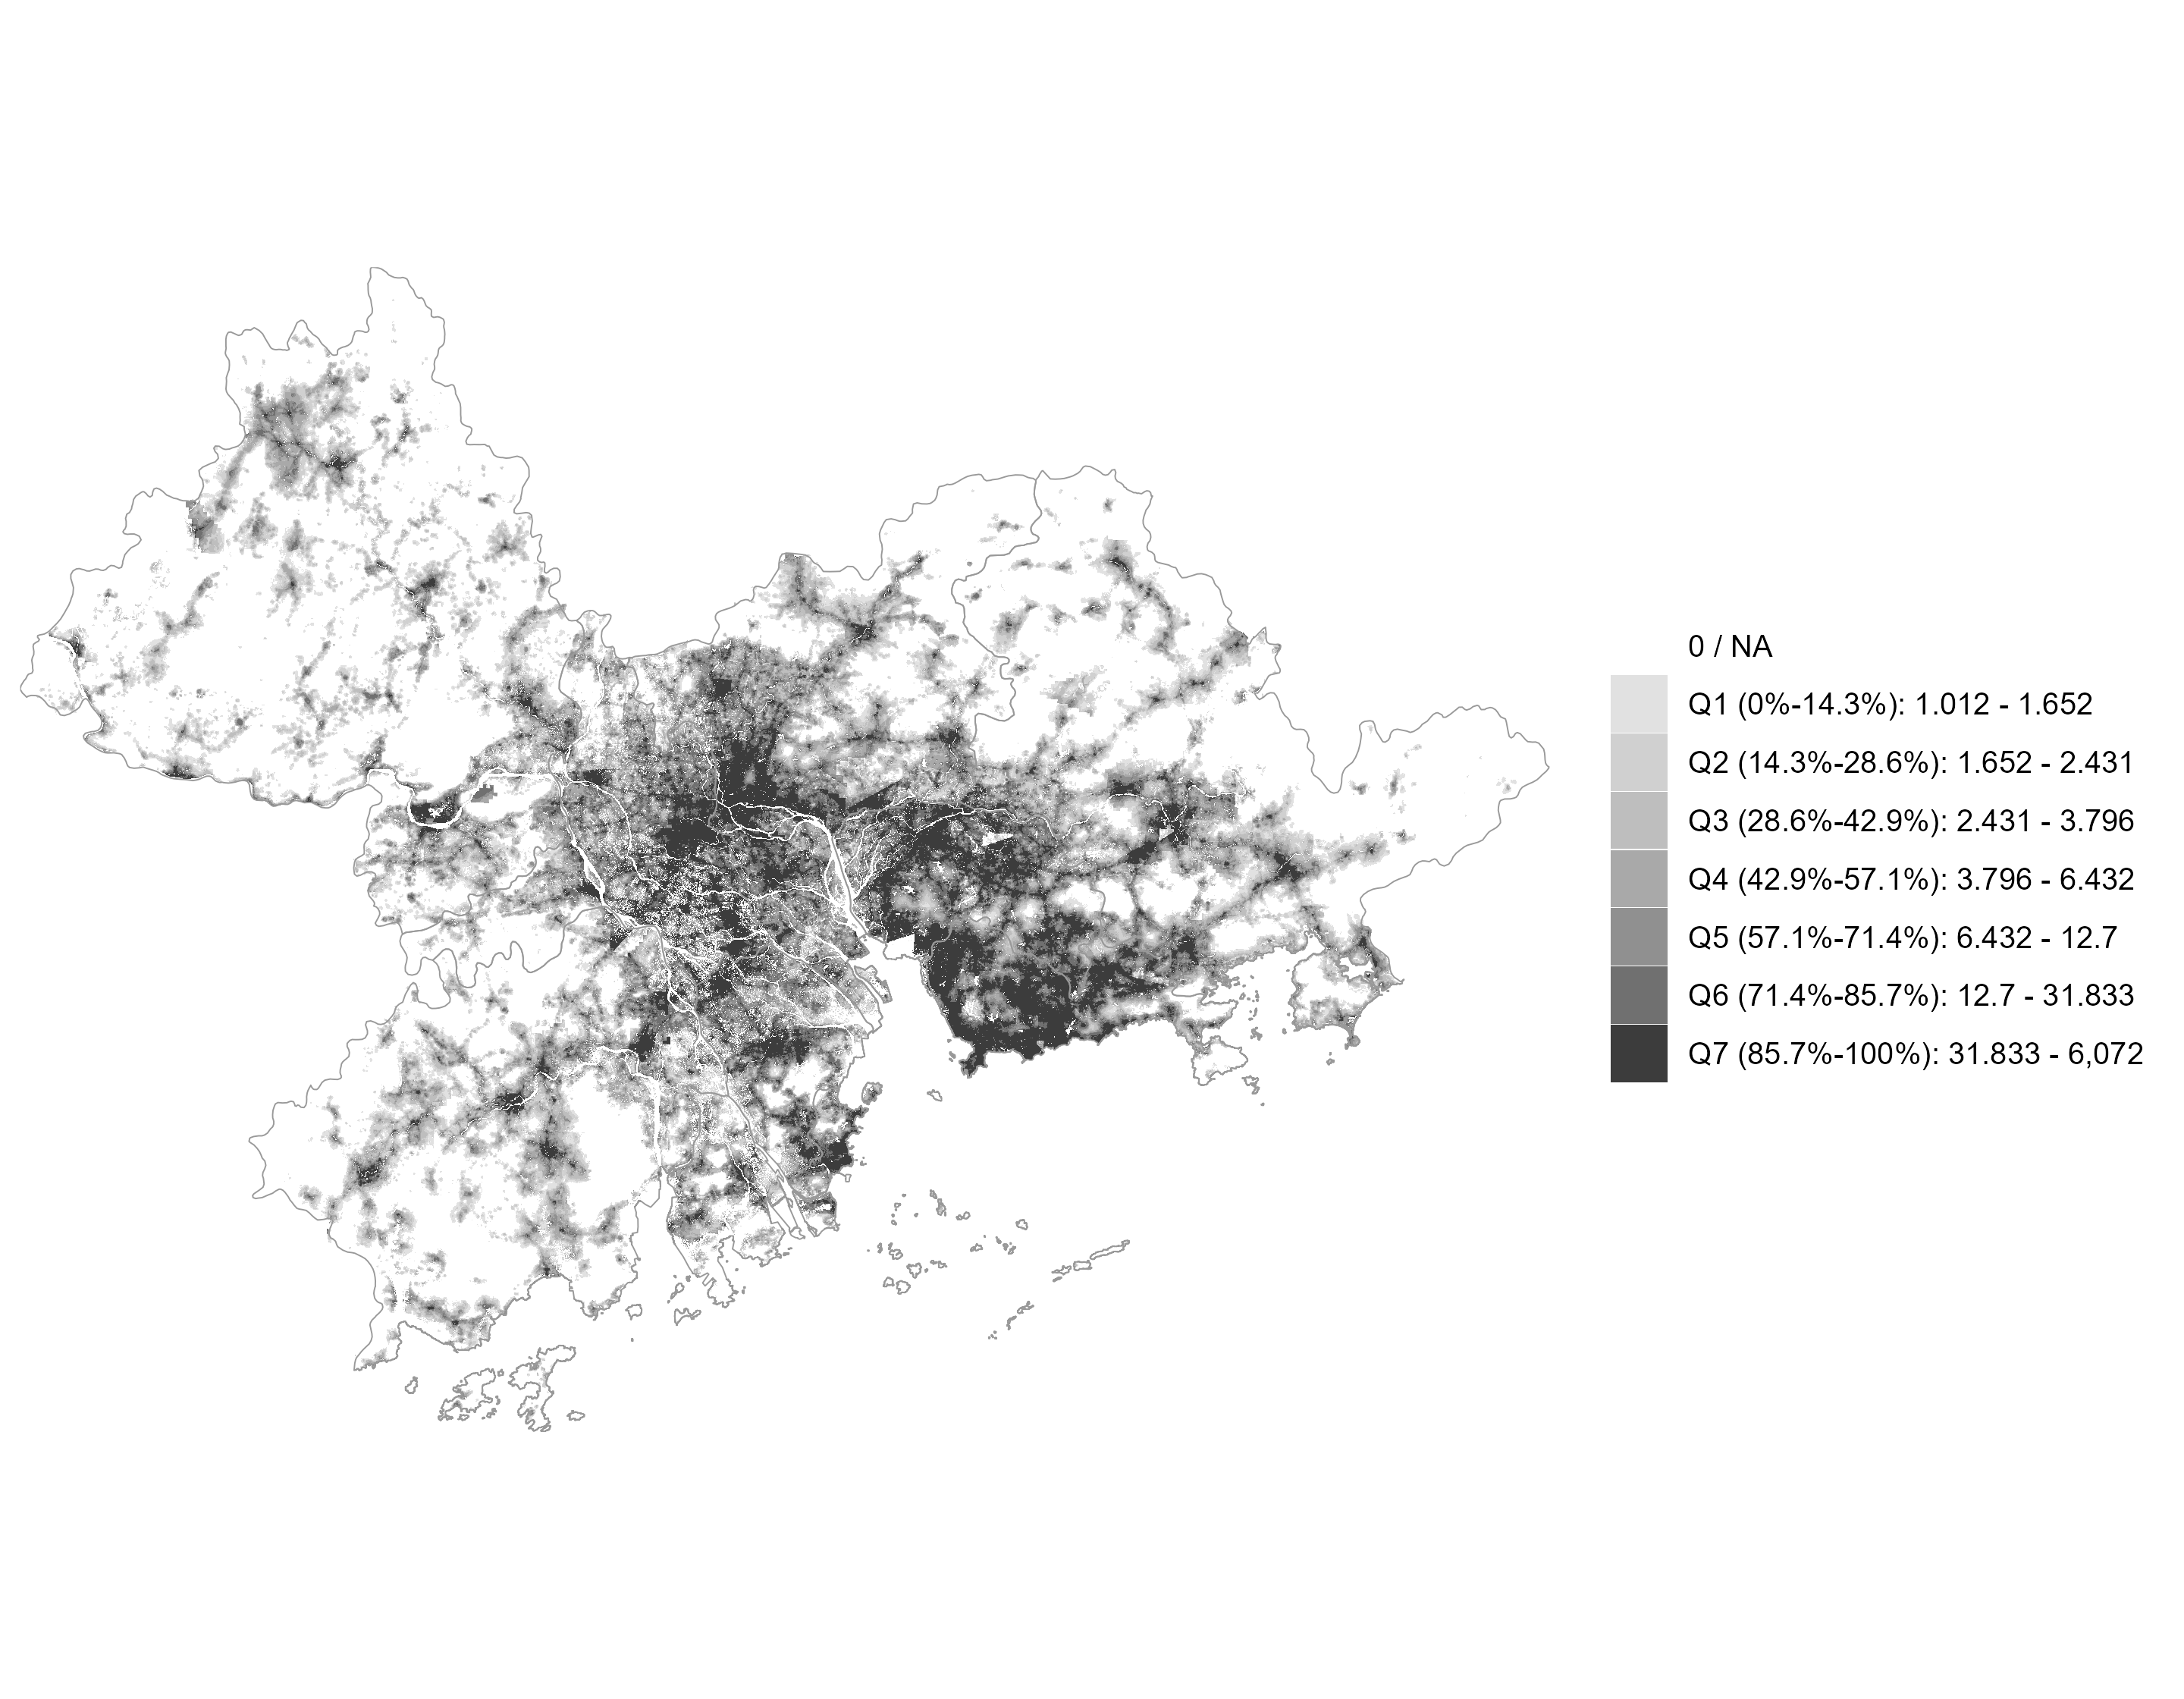
\includegraphics[width=0.95\textwidth]{1.描述性证据/分布图/prd_prefer500m_pop.png}
\caption{2015--2020年珠三角人口分布图}
\label{fig:map_pop}
\end{figure}

\begin{figure}[H]
\centering
\IfFileExists{UV_shape.png}{\includegraphics[width=\textwidth]{UV_shape.png}}{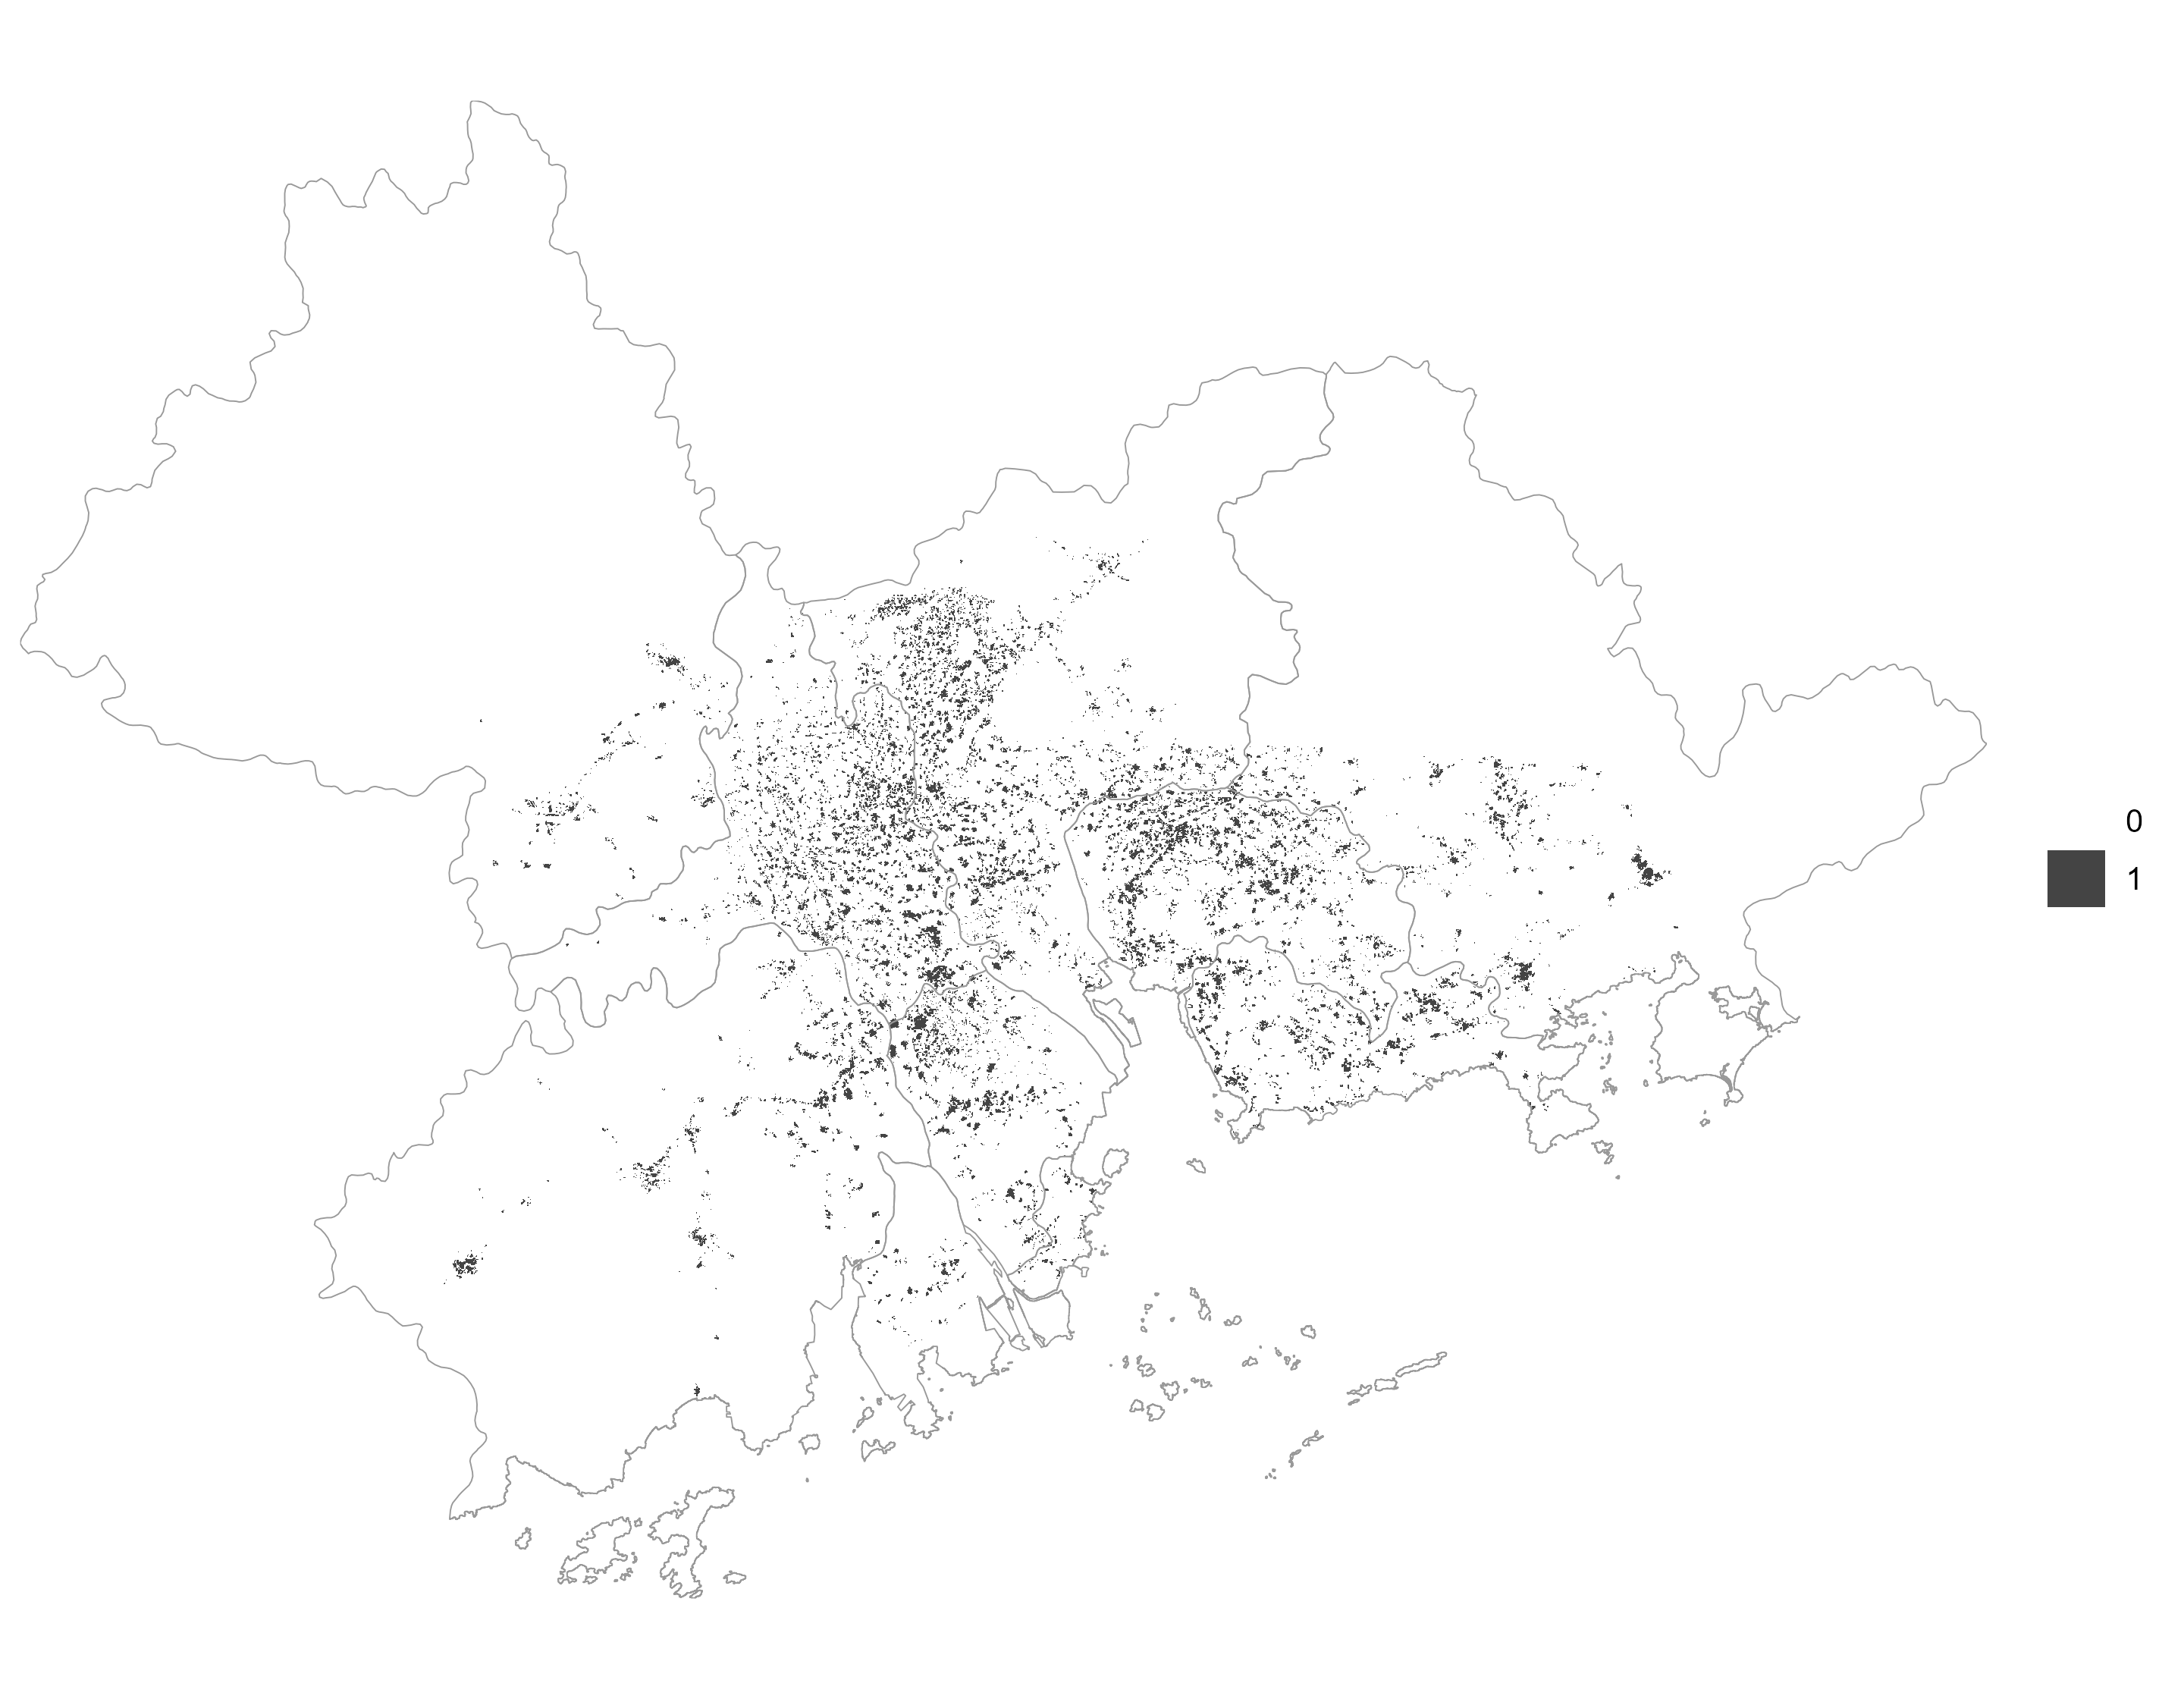
\includegraphics[width=\textwidth]{1.描述性证据/分布图/prd_prefer500m_urban_village.png}}
\caption{城中村空间形态与100米网格尺度示意}
\label{fig:uv_scale}
\end{figure}

\begin{figure}[H]
\centering
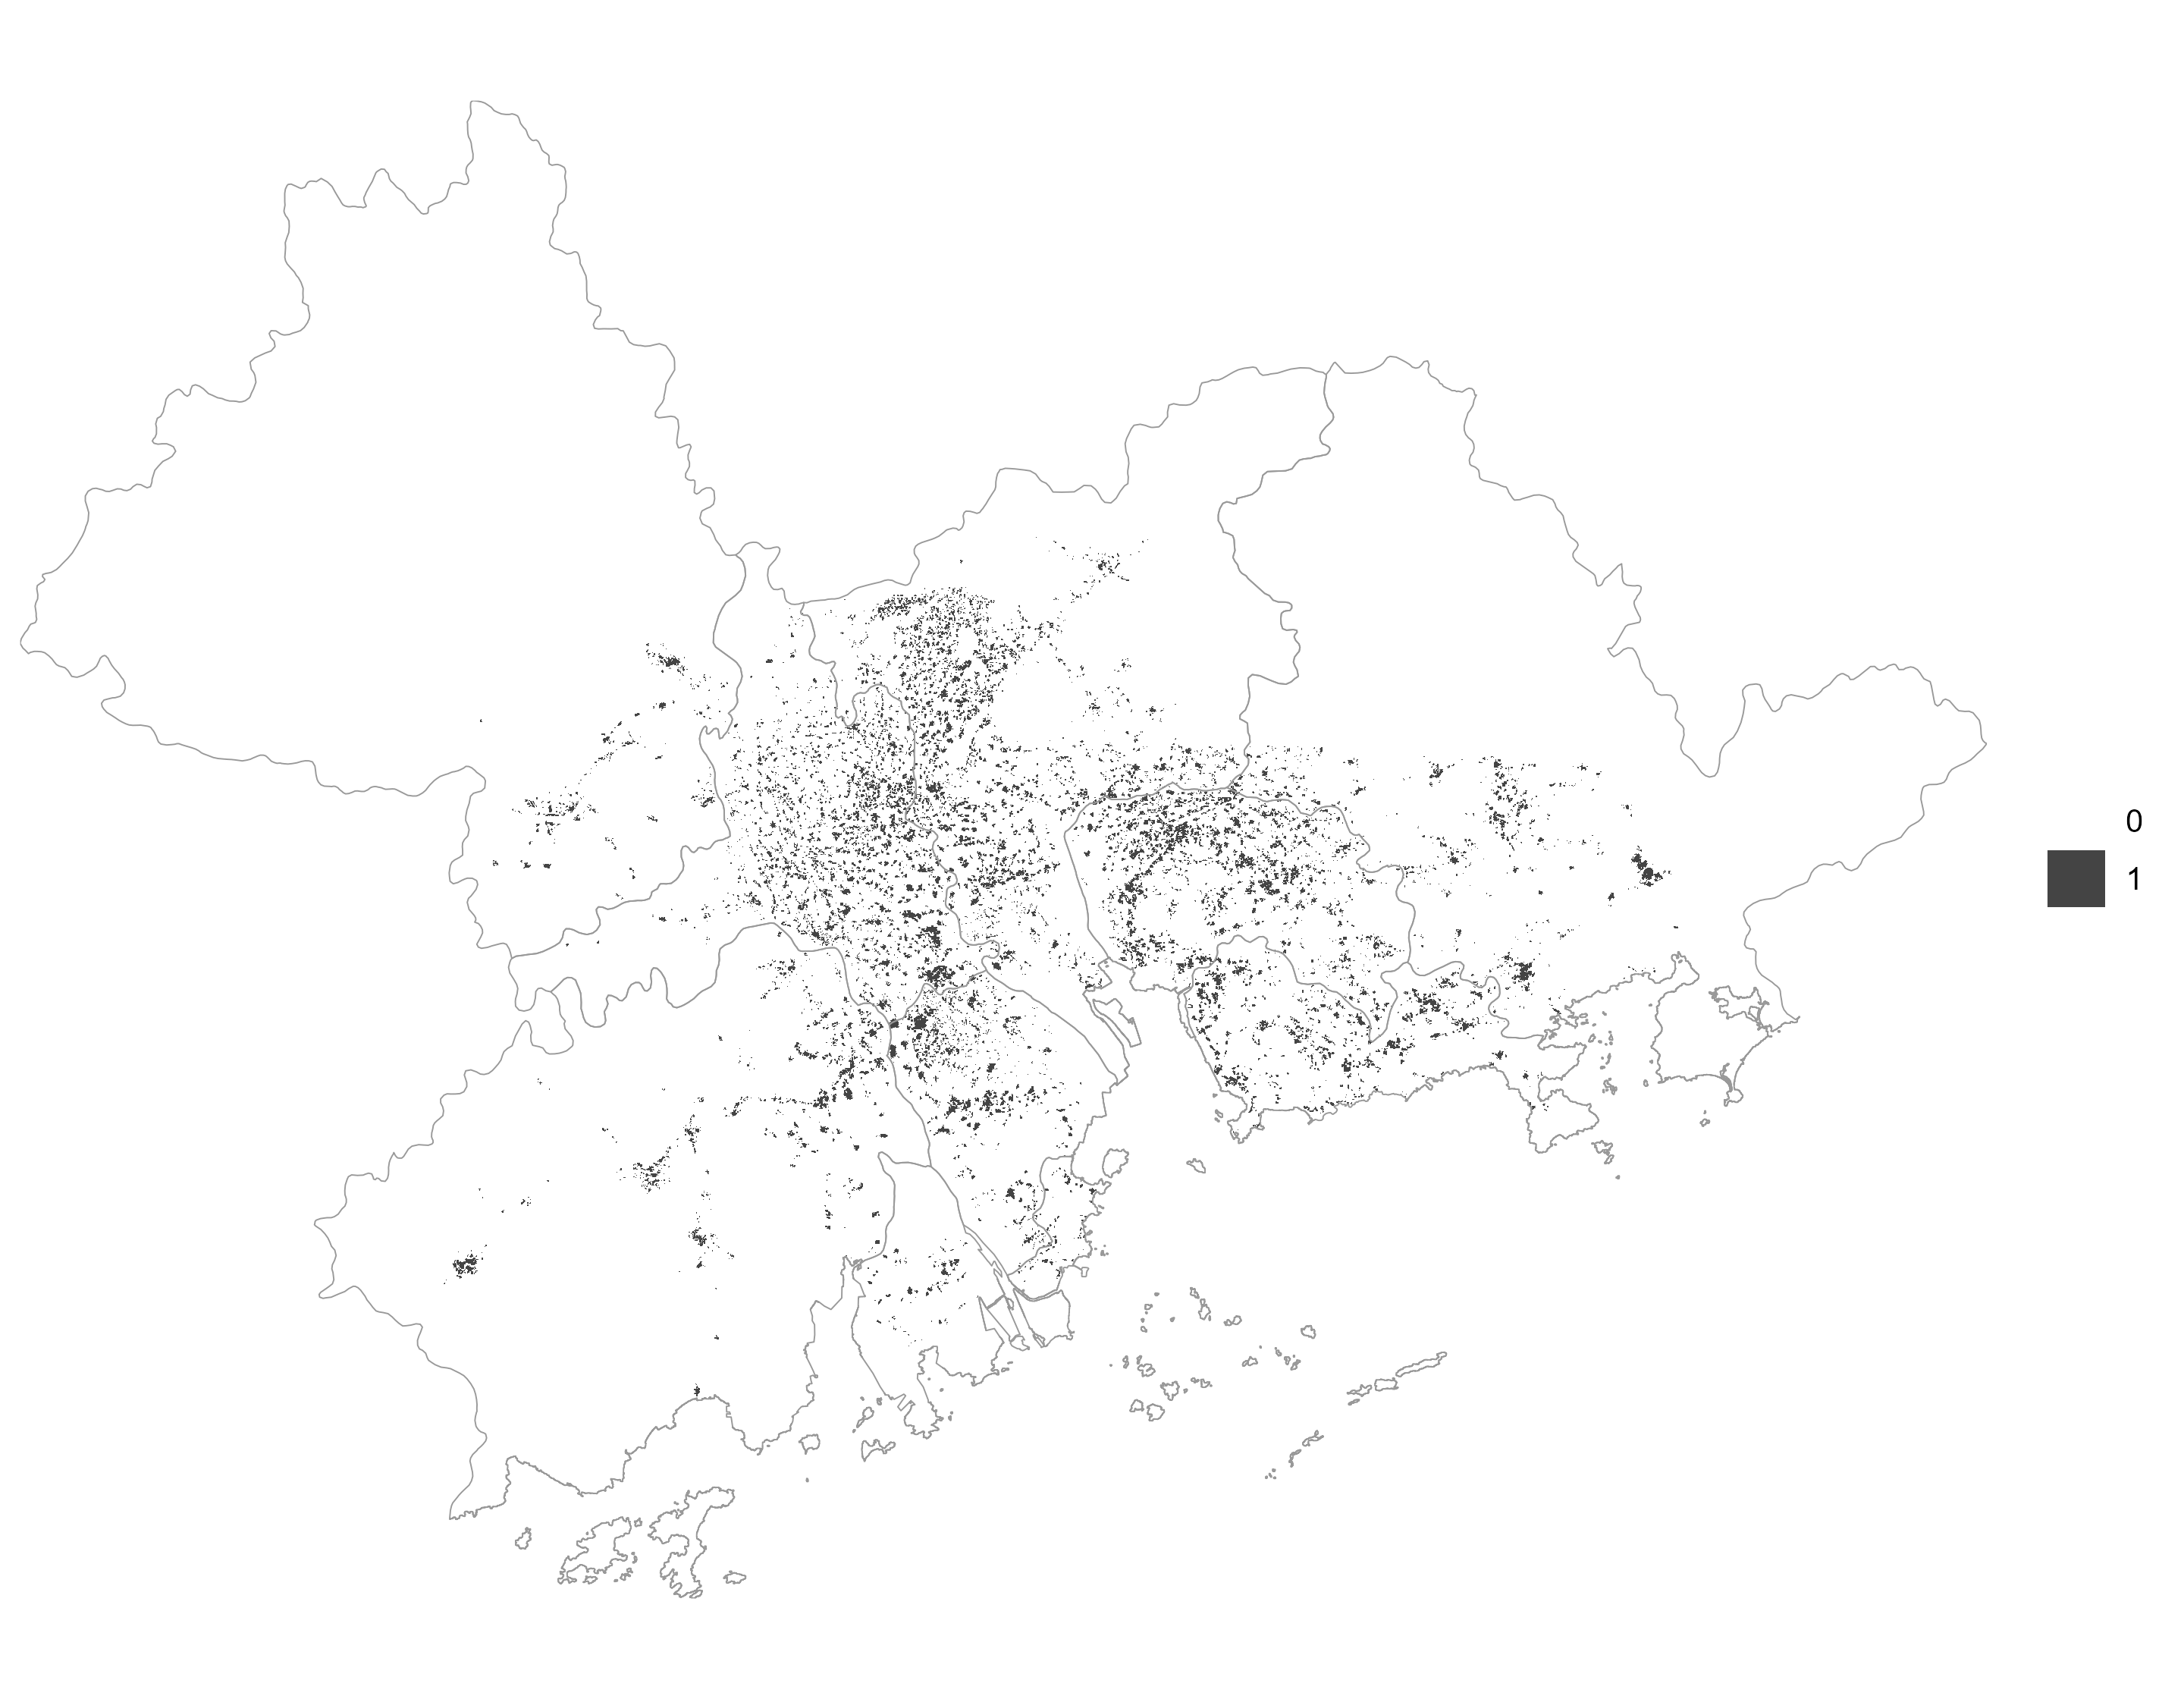
\includegraphics[width=\textwidth]{1.描述性证据/分布图/prd_prefer500m_urban_village.png}
\caption{2018年珠三角城中村分布图}
\label{fig:map_uv_old}
\end{figure}

\begin{table}[H]
\centering
\caption{关税清单匹配与样本规模}
\label{tab:tariff_match}
\zihao{5}
\begin{tabular*}{\textwidth}{@{\extracolsep{\fill}}lr}
\toprule
匹配项目 & 数量 \\
\midrule
8位编码直接匹配（以00结尾的中国HS-8与HTSUS-8） & 21,985 \\
6位编码匹配（以HS-6与HTSUS前6位匹配） & 40,390 \\
未匹配到关税清单的记录 & 32,254 \\
2016年进出口记录（完成地理编码） & 2,971,121 \\
\bottomrule
\end{tabular*}
\end{table}

\begin{table}[H]
\centering
\caption{基础设施可达性指标的分类口径与POI关键词集合}
\label{tab:infra_access}
\zihao{5}
\begin{adjustbox}{width=\textwidth}
\begin{tabular}{p{3.2cm} p{3.2cm} p{7.9cm}}
\toprule
维度 & 指标（最近距离） & POI关键词集合（不删减） \\
\midrule
交通可达性 & 公交站 & 公交车站 \\
交通可达性 & 地铁站 & 地铁站 \\
\midrule
教育可达性 & 幼儿园 & 幼儿园 \\
教育可达性 & 小学 & 小学 \\
教育可达性 & 中学 & 中学 \\
教育可达性 & 职业学校 & 职业学校 \\
教育可达性 & 大学 & 大学 \\
\midrule
医疗可达性 & 初级医疗服务点 & `诊所', `卫生院', `疾病预防' \\
医疗可达性 & 中级医疗服务点 & `综合医院', `专科医院', `口腔医院', `骨科医院', `妇科医院', `眼科医院', `精神病医院', `肿瘤医院', `传染病医院', `脑科医院', `耳鼻喉医院', `胸科医院' \\
医疗可达性 & 高级医疗服务点 & `三级甲等医院', `急救中心' \\
\midrule
金融可达性 & 地方性金融机构 & `银行', `农村商业银行', `金融保险机构', `上海农商银行', `上海银行', `北京银行', `深圳农村商业银行', `财务公司', `北京农商银行', `广州农商银行', `上海浦东发展银行' \\
金融可达性 & 全国性股份制商业银行 & `招商银行', `上海浦东发展银行', `中信银行', `中国光大银行', `华夏银行', `中国民生银行', `广发银行', `兴业银行', `平安银行', `浙商银行', `恒丰银行', `渤海银行' \\
金融可达性 & 国有商业银行 & `中国工商银行', `中国农业银行', `中国银行', `中国建设银行', `交通银行', `中国邮政储蓄银行' \\
\bottomrule
\end{tabular}
\end{adjustbox}
\end{table}

\subsection{城中村特征变量说明}
本文在解释性分析中进一步构造了餐馆密度、菜系熵、基础设施可达性和住房市场代理变量，以刻画城中村周边的社会互动结构、公共服务环境和居住成本条件。

本文使用2017年高德地图POI数据识别餐馆位置，并以街道层面餐馆数量除以街道面积构造餐馆密度指标。餐馆等低门槛、高频共在的消费性场所可被理解为塑造日常互动与社会支持网络的“会面机会结构”，从而与地缘支持网络的强度相关\citep{feld1981foci, mcpherson2001birds, oldenburg1999great, klinenberg2018palaces, granovetter1973strength}。考虑到高德POI中存在相当比例餐饮点位缺乏明确的菜系标注，本文在计算餐馆密度时仅保留能够被可靠分类的餐馆，以避免将便利店、无明确菜系的小吃摊等难以对应“地缘社会网络支持”功能的点位机械纳入。

菜系信息熵是本文机制分析的重要变量之一，用以刻画街道层面地缘网络的多样性。鉴于高德POI中大量餐饮点位缺少菜系标签，本文基于餐馆名称构造菜系分类器，并在街道层面计算熵指标。具体而言，本文先在LLM辅助下为18个主要菜系构建种子词表，再采用seeded-LDA（带种子约束的主题模型）对餐馆名称进行建模，以“菜系”为主题训练得到每个餐馆名称属于各主题的概率分布。为确保分类结果具有足够置信度，本文剔除“最大主题概率”低于15\%的餐馆；在18个菜系下，随机分配的最大概率期望约为$1/18\approx5.6\%$，因此15\%阈值意味着最大概率至少达到随机分配的约2.7倍。对保留样本，本文将最大概率对应的主题作为该餐馆的预测菜系，并在街道层面据此计算Shannon信息熵。较高的菜系熵意味着餐饮生态位更为多元且分布更均衡，进而可能对应更高的跨群体接触机会与桥接关系生成概率。

\begin{figure}[H]
\centering

\includegraphics[width=0.95\textwidth]{1.描述性证据/lda_topic_wordclouds_multiyear_grid_3x6.png}
\caption{菜系主题词云图}
\label{fig:lda_wordclouds}
\end{figure}

\begin{figure}[H]
\centering
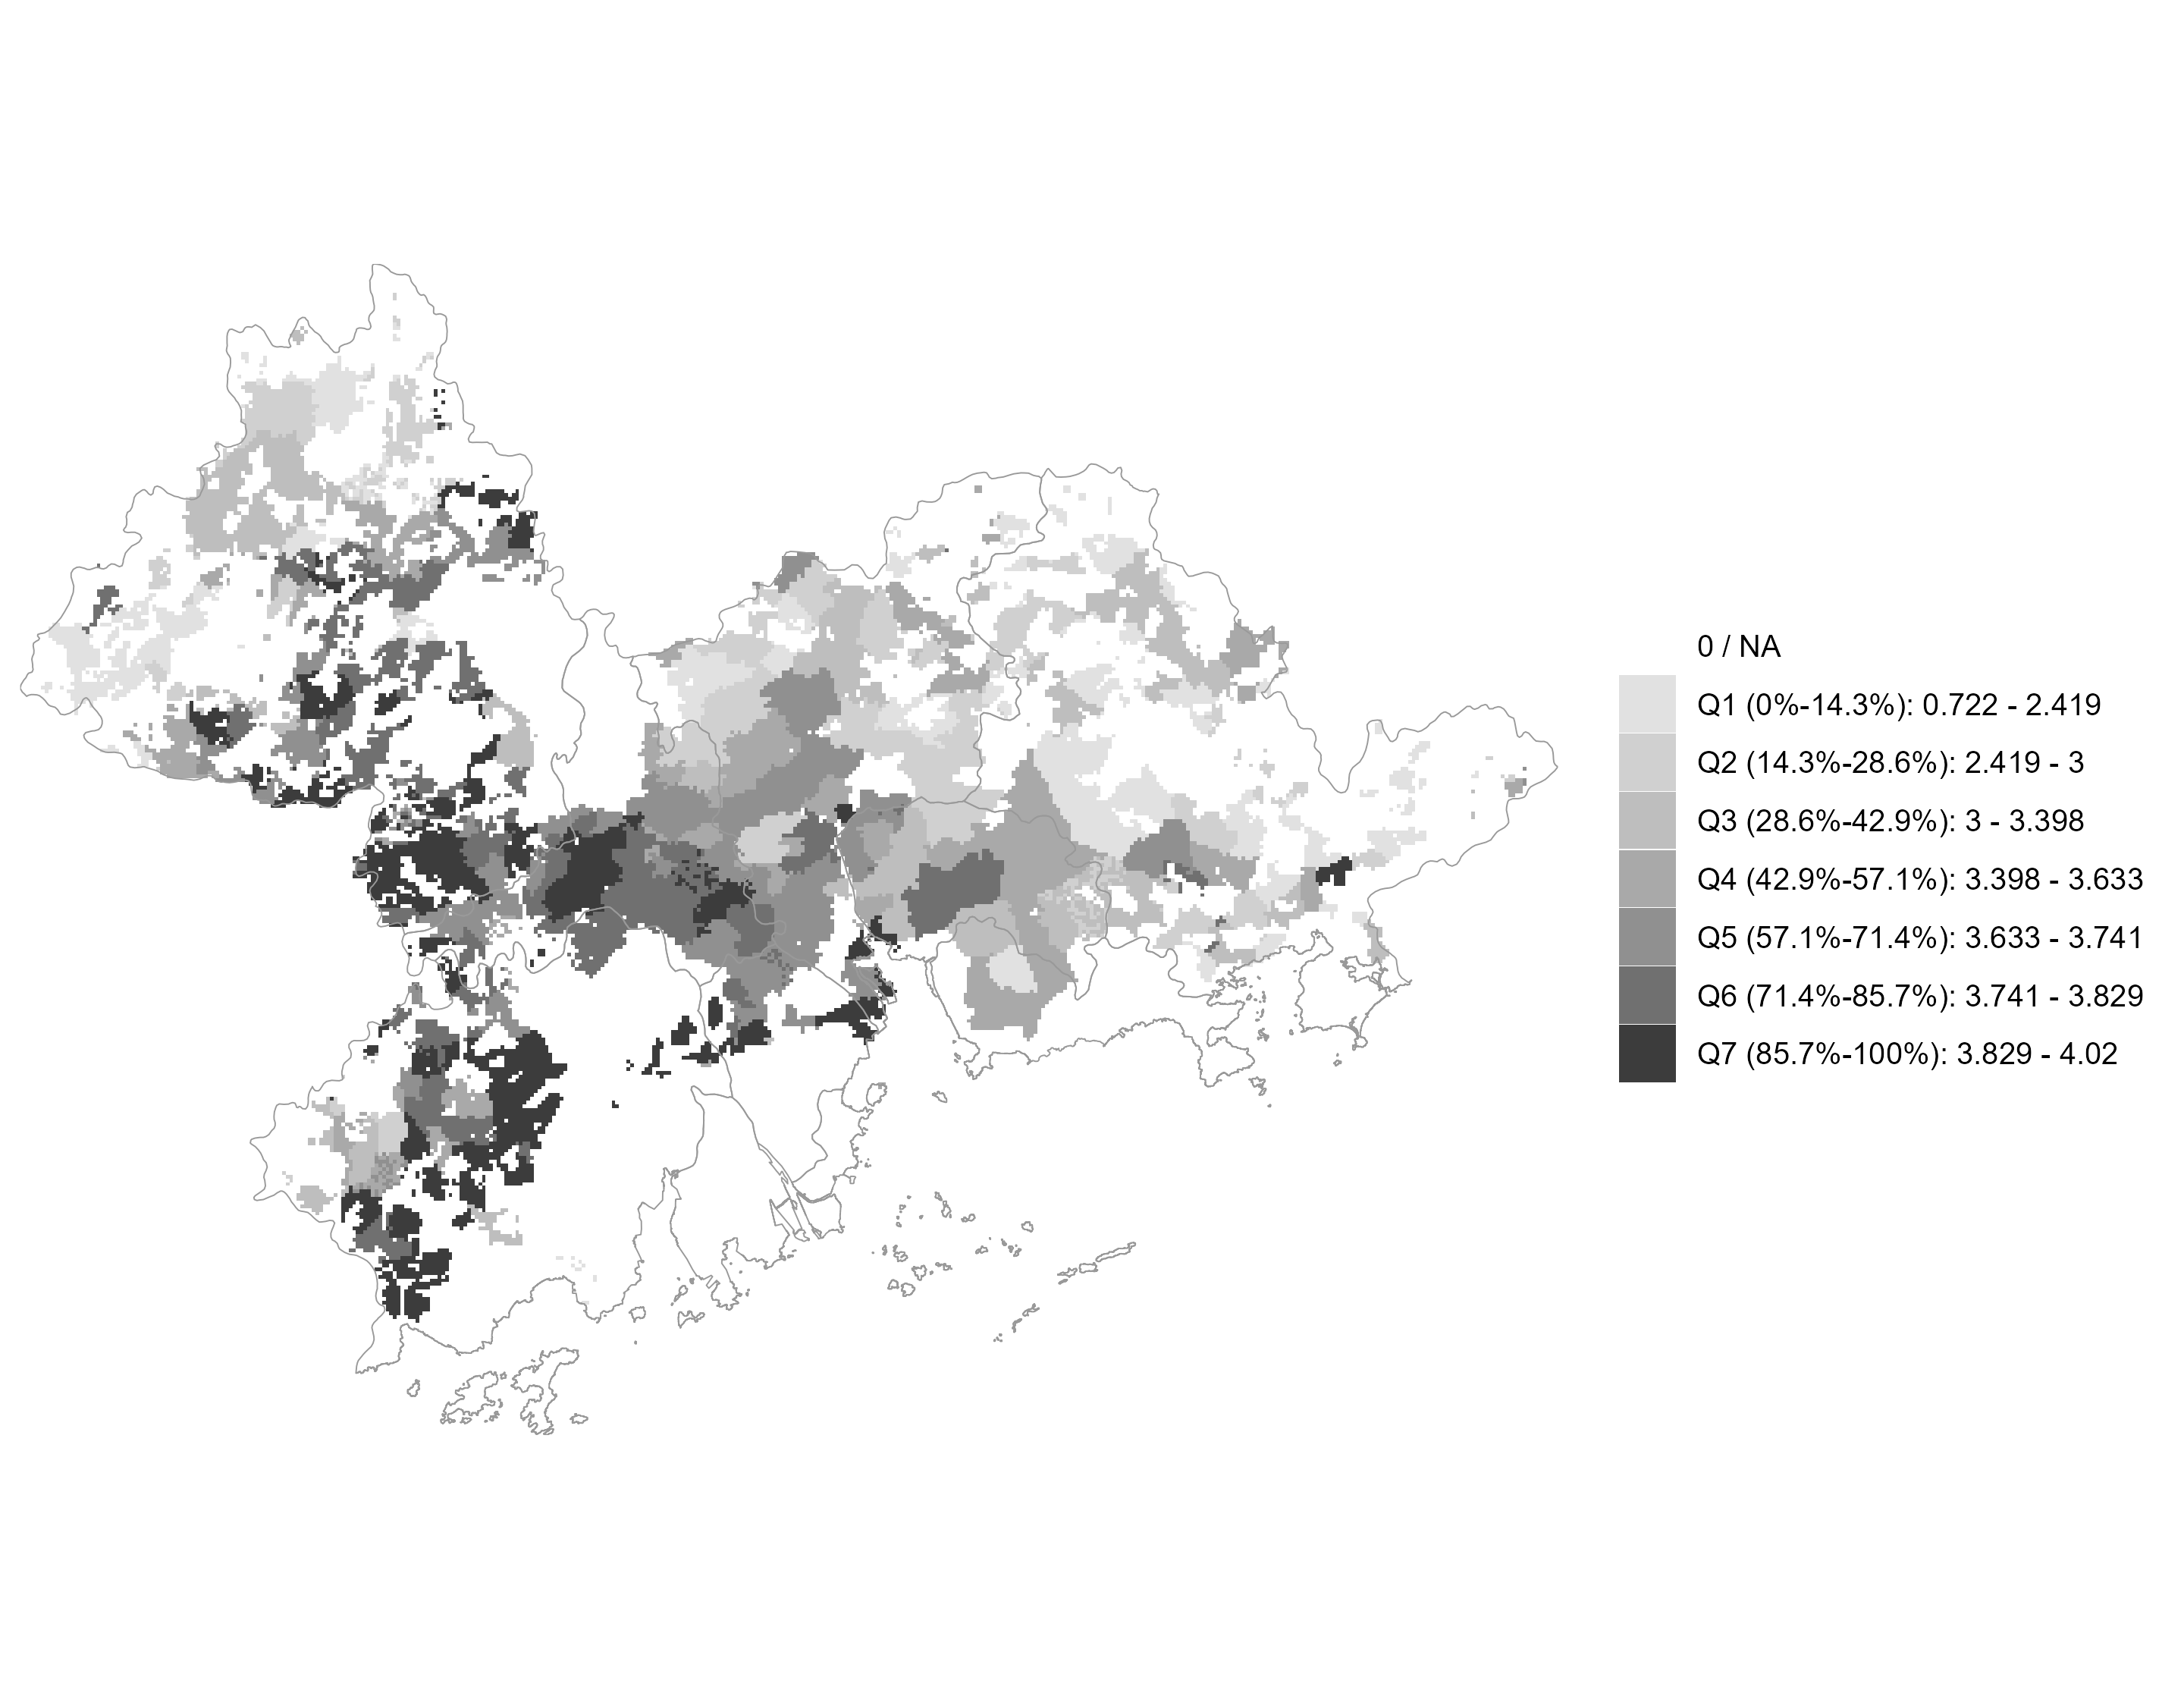
\includegraphics[width=0.95\textwidth]{1.描述性证据/分布图/prd_prefer500m_cuisine_entropy_2017.png}
\caption{2017年珠三角菜系熵分布图}
\label{fig:map_entropy}
\end{figure}

本文进一步根据OpenStreetMap和高德POI数据构造基础设施可达性指标。具体做法是：以100m网格质心为参考点，分别计算到公交站、地铁站、教育设施、医疗设施和金融机构的最短距离，以刻画城中村周边公共服务供给与空间可达性。由于分类口径较为细致，全部指标及对应POI关键词集合汇总见附录表 \ref{tab:infra_access}。

本文还以二手房市场信息作为居住成本的代理变量。由于城中村内部租赁市场的租金数据难以系统获取，本文参考住房经济学中“住房服务价值/隐含租金”的思路，将二手房市场价格作为居住成本的代理信息来源。住房资产价格在均衡中与住房服务流（租金或隐含租金）存在紧密联系，相关框架与经验证据表明房价能够反映居住成本与住房服务价值的空间差异\citep{gallin2004rents, himmelberg2005assessing, gindelsky2019valuing, loewenstein2023prices, bls2025oer}。在操作层面，本文从链家获取二手房挂牌信息，按半年度计算住宅小区挂牌均价；对每一个城中村网格，选取距离最近的三个住宅小区并取其半年度挂牌均价的均值，作为该网格的居住成本代理变量。该做法旨在刻画局部住房市场价格水平，并通过邻近小区聚合降低单一小区价格噪声与样本稀疏带来的测度误差。

\begin{table}[H]
\centering
\caption{中心、外围城中村与正规街区的基线特征比较}
\label{tab:baseline}
\zihao{5}
\begin{adjustbox}{width=\textwidth,center}
\begin{tabular}{lcccccc}
\toprule
 & \multicolumn{1}{c}{正规街区} & \multicolumn{1}{c}{中心城中村} & \multicolumn{1}{c}{外围城中村} & \multicolumn{1}{c}{\makecell{中心城中村\\$-$正规街区}} & \multicolumn{1}{c}{\makecell{外围城中村\\$-$正规街区}} & \multicolumn{1}{c}{\makecell{外围城中村\\$-$中心城中村}} \\
变量 & \makecell{均值\\（标准差）} & \makecell{均值\\（标准差）} & \makecell{均值\\（标准差）} & \makecell{差异\\{[标准误]}} & \makecell{差异\\{[标准误]}} & \makecell{差异\\{[标准误]}} \\
\midrule
对美出口关税暴露度 & \makecell{0.024\\(0.008)} & \makecell{0.025\\(0.008)} & \makecell{0.027\\(0.012)} & \makecell{0.000\\ {[0.001]}} & \makecell{0.003\\ {[0.002]}} & \makecell{0.002\\ {[0.002]}} \\
人口 & \makecell{52.472\\(91.110)} & \makecell{70.732\\(87.471)} & \makecell{34.447\\(43.502)} & \makecell{18.260***\\ {[4.096]}} & \makecell{-18.026***\\ {[5.610]}} & \makecell{-36.286***\\ {[7.059]}} \\
每十万人犯罪率 & \makecell{28.899\\(1701.196)} & \makecell{60.328\\(1394.211)} & \makecell{69.167\\(5166.667)} & \makecell{31.429***\\ {[5.175]}} & \makecell{40.269***\\ {[13.864]}} & \makecell{8.839\\ {[13.918]}} \\
城中村面积占比（\%） & \makecell{0.000\\(0.000)} & \makecell{51.796\\(35.467)} & \makecell{44.543\\(34.383)} & \makecell{51.796***\\ {[0.741]}} & \makecell{44.543***\\ {[1.268]}} & \makecell{-7.254***\\ {[1.157]}} \\
事前挂牌单价 & \makecell{22665.572\\(16472.584)} & \makecell{23708.588\\(23651.887)} & \makecell{24509.496\\(15446.251)} & \makecell{1043.017\\ {[1155.318]}} & \makecell{1843.924\\ {[2238.459]}} & \makecell{800.907\\ {[2577.787]}} \\
到公交站距离（米） & \makecell{5198.428\\(4806.062)} & \makecell{5625.248\\(5146.610)} & \makecell{9779.328\\(9184.721)} & \makecell{426.821\\ {[439.411]}} & \makecell{4580.901***\\ {[1586.672]}} & \makecell{4154.080**\\ {[1725.681]}} \\
到地铁站距离（米） & \makecell{24642.578\\(18407.000)} & \makecell{23914.184\\(18387.453)} & \makecell{39613.570\\(26248.330)} & \makecell{-728.393\\ {[1080.789]}} & \makecell{14970.993***\\ {[4551.986]}} & \makecell{15699.387***\\ {[4483.359]}} \\
到幼儿园距离（米） & \makecell{939.502\\(723.617)} & \makecell{484.669\\(454.660)} & \makecell{932.266\\(1005.905)} & \makecell{-454.833***\\ {[35.880]}} & \makecell{-7.236\\ {[65.250]}} & \makecell{447.597***\\ {[60.693]}} \\
到小学距离（米） & \makecell{1201.118\\(774.720)} & \makecell{723.624\\(559.141)} & \makecell{965.778\\(770.205)} & \makecell{-477.494***\\ {[46.250]}} & \makecell{-235.340***\\ {[70.951]}} & \makecell{242.154***\\ {[46.848]}} \\
到中学距离（米） & \makecell{1591.266\\(1079.392)} & \makecell{1195.921\\(884.755)} & \makecell{1640.236\\(1199.428)} & \makecell{-395.345***\\ {[42.085]}} & \makecell{48.971\\ {[82.843]}} & \makecell{444.316***\\ {[80.594]}} \\
到高等教育机构距离（米） & \makecell{3500.604\\(2650.534)} & \makecell{3108.148\\(2344.231)} & \makecell{5992.325\\(4629.864)} & \makecell{-392.456***\\ {[144.122]}} & \makecell{2491.721***\\ {[569.554]}} & \makecell{2884.177***\\ {[549.843]}} \\
到职业教育机构距离（米） & \makecell{2526.431\\(1826.389)} & \makecell{2123.993\\(1573.893)} & \makecell{3807.838\\(3206.503)} & \makecell{-402.438***\\ {[90.388]}} & \makecell{1281.407***\\ {[368.156]}} & \makecell{1683.845***\\ {[367.395]}} \\
到基础医疗机构距离（米） & \makecell{737.618\\(549.633)} & \makecell{373.767\\(328.002)} & \makecell{615.264\\(579.920)} & \makecell{-363.851***\\ {[23.457]}} & \makecell{-122.354***\\ {[34.844]}} & \makecell{241.497***\\ {[33.733]}} \\
到中级医疗机构距离（米） & \makecell{1756.764\\(1314.548)} & \makecell{1288.277\\(1102.159)} & \makecell{1987.414\\(1674.319)} & \makecell{-468.487***\\ {[62.871]}} & \makecell{230.650*\\ {[119.503]}} & \makecell{699.137***\\ {[110.555]}} \\
到高级医疗机构距离（米） & \makecell{3440.906\\(2202.146)} & \makecell{2985.483\\(2118.469)} & \makecell{6310.334\\(6481.816)} & \makecell{-455.423***\\ {[125.912]}} & \makecell{2869.428***\\ {[867.716]}} & \makecell{3324.851***\\ {[869.899]}} \\
到中小银行网点距离（米） & \makecell{811.466\\(626.221)} & \makecell{455.505\\(386.498)} & \makecell{802.269\\(784.195)} & \makecell{-355.961***\\ {[34.037]}} & \makecell{-9.197\\ {[63.481]}} & \makecell{346.764***\\ {[57.159]}} \\
到股份制银行网点距离（米） & \makecell{2909.621\\(2315.002)} & \makecell{2482.858\\(2078.705)} & \makecell{7201.306\\(7052.067)} & \makecell{-426.762***\\ {[124.483]}} & \makecell{4291.686***\\ {[970.713]}} & \makecell{4718.448***\\ {[977.376]}} \\
到国有银行网点距离（米） & \makecell{1526.952\\(1179.928)} & \makecell{1059.562\\(898.190)} & \makecell{1668.049\\(1442.971)} & \makecell{-467.390***\\ {[61.757]}} & \makecell{141.097\\ {[115.584]}} & \makecell{608.487***\\ {[100.029]}} \\
事前夜光（对数） & \makecell{4.109\\(0.070)} & \makecell{4.116\\(0.056)} & \makecell{3.926\\(0.227)} & \makecell{0.007**\\ {[0.003]}} & \makecell{-0.183***\\ {[0.026]}} & \makecell{-0.190***\\ {[0.026]}} \\
菜系熵 & \makecell{3.349\\(0.603)} & \makecell{3.373\\(0.530)} & \makecell{3.355\\(0.739)} & \makecell{0.024\\ {[0.047]}} & \makecell{0.005\\ {[0.110]}} & \makecell{-0.019\\ {[0.091]}} \\
餐馆数量 & \makecell{259.276\\(361.245)} & \makecell{277.480\\(385.859)} & \makecell{568.599\\(744.746)} & \makecell{18.204\\ {[27.593]}} & \makecell{309.323**\\ {[139.520]}} & \makecell{291.119**\\ {[137.704]}} \\
餐馆密度 & \makecell{0.057\\(0.152)} & \makecell{0.059\\(0.139)} & \makecell{0.101\\(0.160)} & \makecell{0.002\\ {[0.007]}} & \makecell{0.044*\\ {[0.026]}} & \makecell{0.042\\ {[0.025]}} \\
\bottomrule
\end{tabular}
\end{adjustbox}
\end{table}

\section{额外的稳健性检验}

\begin{table}[H]
\centering
\caption{稳健性 标准误聚类口径}
\label{tab:robust_se}
\zihao{5}
\begin{tabular*}{\textwidth}{@{\extracolsep{\fill}}lc}
\toprule
聚类口径 & $Post\times Exposure$ \\
\midrule
县（区）聚类 & \makecell{0.210***\\(0.081)} \\
城市聚类 & \makecell{0.210***\\(0.050)} \\
网格$\times$城市$\times$半年度聚类 & \makecell{0.176**\\(0.070)} \\
\bottomrule
\end{tabular*}
\vspace{0.2cm}

\par\raggedright\zihao{5} 注：表中为$Post\times Exposure$的系数，括号内为聚类标准误。+ $p<0.15$，* $p<0.10$，** $p<0.05$，*** $p<0.01$。
\end{table}

\begin{table}[H]
\centering
\caption{稳健性 对极端值缩尾}
\label{tab:robust_winsor}
\zihao{5}
\begin{tabular*}{\textwidth}{@{\extracolsep{\fill}}lc}
\toprule
设定 & $Post\times Exposure$ \\
\midrule
基准 & \makecell{0.210***\\(0.081)} \\
1\%--99\%缩尾 & \makecell{0.210***\\(0.081)} \\
95\%缩尾 & \makecell{0.176**\\(0.070)} \\
\bottomrule
\end{tabular*}
\vspace{0.2cm}

\par\raggedright\zihao{5} 注：表中为$Post\times Exposure$的系数。+ $p<0.15$，* $p<0.10$，** $p<0.05$，*** $p<0.01$。
\end{table}

\section{潜在调节效应讨论}
\begin{table}[H]
\centering
\caption{民生设施可达性的调节效应与恢复速度}
\label{tab:mod_infra_level_speed}
\zihao{5}
\resizebox{\textwidth}{!}{
\begin{tabular}{lccccccccc}
\toprule
\multicolumn{1}{c}{调节变量（距离）} & \multicolumn{1}{c}{总犯罪} & \multicolumn{2}{c}{财产型犯罪} & \multicolumn{2}{c}{冲动型犯罪} & \multicolumn{2}{c}{企业犯罪} & \multicolumn{2}{c}{地下经济犯罪} \\
\cmidrule(lr){2-2}\cmidrule(lr){3-4}\cmidrule(lr){5-6}\cmidrule(lr){7-8}\cmidrule(lr){9-10}
 & $b_{level}$ & $b_{level}$ & $b_{speed,mod}$ & $b_{level}$ & $b_{speed,mod}$ & $b_{level}$ & $b_{speed,mod}$ & $b_{level}$ & $b_{speed,mod}$ \\
\midrule
到公交站距离 & \makecell{-0.068**\\(0.032)} & \makecell{-0.047\\(0.046)} & \makecell{0.013\\(0.036)} & \makecell{0.024\\(0.059)} & \makecell{0.013\\(0.023)} & \makecell{-0.045\\(0.105)} & \makecell{-0.012\\(0.054)} & \makecell{-0.015\\(0.044)} & \makecell{0.016\\(0.040)} \\
到地铁站距离 & \makecell{-0.040\\(0.125)} & \makecell{-0.098\\(0.119)} & \makecell{0.192***\\(0.050)} & \makecell{0.065\\(0.155)} & \makecell{0.226***\\(0.063)} & \makecell{-0.528**\\(0.220)} & \makecell{0.182*\\(0.109)} & \makecell{-0.121\\(0.143)} & \makecell{0.291***\\(0.051)} \\
到幼儿园距离 & \makecell{-0.094\\(0.080)} & \makecell{-0.153\\(0.143)} & \makecell{0.023\\(0.081)} & \makecell{-0.042\\(0.117)} & \makecell{0.038\\(0.044)} & \makecell{-0.059\\(0.156)} & \makecell{-0.218*\\(0.131)} & \makecell{0.050\\(0.092)} & \makecell{0.074\\(0.060)} \\
到小学距离 & \makecell{-0.284***\\(0.099)} & \makecell{-0.293**\\(0.122)} & \makecell{0.101**\\(0.048)} & \makecell{-0.171\\(0.104)} & \makecell{0.044\\(0.052)} & \makecell{-0.364**\\(0.163)} & \makecell{-0.162\\(0.123)} & \makecell{-0.293**\\(0.116)} & \makecell{0.105\\(0.069)} \\
到中学距离 & \makecell{-0.168*\\(0.090)} & \makecell{-0.094\\(0.150)} & \makecell{0.052\\(0.044)} & \makecell{-0.223**\\(0.102)} & \makecell{0.112**\\(0.051)} & \makecell{-0.104\\(0.159)} & \makecell{0.036\\(0.116)} & \makecell{-0.310**\\(0.134)} & \makecell{0.076\\(0.078)} \\
到大学距离 & \makecell{-0.134*\\(0.071)} & \makecell{-0.122\\(0.084)} & \makecell{-0.022\\(0.036)} & \makecell{-0.138**\\(0.054)} & \makecell{0.032\\(0.021)} & \makecell{-0.013\\(0.083)} & \makecell{-0.058\\(0.056)} & \makecell{-0.149**\\(0.075)} & \makecell{0.033\\(0.060)} \\
到职业学校距离 & \makecell{-0.169\\(0.117)} & \makecell{-0.071\\(0.113)} & \makecell{-0.025\\(0.033)} & \makecell{-0.122*\\(0.068)} & \makecell{0.055**\\(0.023)} & \makecell{-0.193**\\(0.095)} & \makecell{-0.015\\(0.077)} & \makecell{-0.281\\(0.179)} & \makecell{-0.077\\(0.066)} \\
到初级医疗服务点距离 & \makecell{-0.503***\\(0.175)} & \makecell{-0.093\\(0.113)} & \makecell{0.058\\(0.086)} & \makecell{-0.362**\\(0.169)} & \makecell{-0.018\\(0.099)} & \makecell{-0.004\\(0.237)} & \makecell{-0.118\\(0.117)} & \makecell{-0.086\\(0.093)} & \makecell{0.099\\(0.085)} \\
到中级医疗服务点距离 & \makecell{-0.142\\(0.113)} & \makecell{-0.127\\(0.181)} & \makecell{0.028\\(0.077)} & \makecell{-0.229*\\(0.118)} & \makecell{-0.002\\(0.056)} & \makecell{-0.267\\(0.229)} & \makecell{0.160\\(0.122)} & \makecell{-0.363*\\(0.195)} & \makecell{0.080\\(0.110)} \\
到高级医疗服务点距离 & \makecell{-0.132\\(0.091)} & \makecell{-0.207\\(0.130)} & \makecell{-0.048\\(0.059)} & \makecell{-0.055\\(0.078)} & \makecell{0.049\\(0.035)} & \makecell{-0.205\\(0.201)} & \makecell{0.047\\(0.126)} & \makecell{-0.222\\(0.155)} & \makecell{-0.094\\(0.085)} \\
到地方性金融机构距离 & \makecell{0.009\\(0.108)} & \makecell{0.058\\(0.118)} & \makecell{0.037\\(0.079)} & \makecell{-0.183\\(0.140)} & \makecell{0.038\\(0.080)} & \makecell{0.285\\(0.202)} & \makecell{-0.111\\(0.120)} & \makecell{0.146\\(0.117)} & \makecell{0.082\\(0.074)} \\
到股份制商业银行距离 & \makecell{-0.252**\\(0.100)} & \makecell{-0.213\\(0.134)} & \makecell{-0.065\\(0.069)} & \makecell{-0.164\\(0.100)} & \makecell{0.025\\(0.036)} & \makecell{-0.013\\(0.150)} & \makecell{0.051\\(0.119)} & \makecell{-0.301**\\(0.138)} & \makecell{-0.151\\(0.103)} \\
到国有商业银行距离 & \makecell{-0.123\\(0.104)} & \makecell{-0.064\\(0.094)} & \makecell{0.055\\(0.045)} & \makecell{-0.066\\(0.107)} & \makecell{0.073\\(0.061)} & \makecell{-0.015\\(0.201)} & \makecell{0.180\\(0.148)} & \makecell{-0.274**\\(0.130)} & \makecell{0.069\\(0.086)} \\
\bottomrule
\end{tabular}}
\vspace{0.2cm}

\par\raggedright\zihao{5} 注：表中同时报告当期水平效应（$b_{level}$：三重交互项$Post\times Exposure\times Dist$的系数）与恢复速度调节效应（$b_{speed,mod}$），样本为100m城中村网格。* $p<0.10$，** $p<0.05$，*** $p<0.01$。
\end{table}

\begin{table}[H]
\centering
\caption{住房市场的调节效应（事前指标：2015H1--2017H2均值）}
\label{tab:mod_house_pre1517}
\zihao{5}
\begin{adjustbox}{width=\textwidth,center}
\begin{tabular}{lcccccccc}
\toprule
\multirow{2}{*}{因变量} & \multicolumn{2}{c}{事前挂牌单价} & \multicolumn{2}{c}{事前成交单价} & \multicolumn{2}{c}{事前成交周期} & \multicolumn{2}{c}{事前价差} \\
\cmidrule(lr){2-3}\cmidrule(lr){4-5}\cmidrule(lr){6-7}\cmidrule(lr){8-9}
  & ntl\_dist & ntl\_only & ntl\_dist & ntl\_only & ntl\_dist & ntl\_only & ntl\_dist & ntl\_only \\
\midrule
总犯罪 & \makecell{0.138*\\(0.075)} & \makecell{0.161**\\(0.078)} & \makecell{0.031\\(0.075)} & \makecell{0.054\\(0.078)} & \makecell{-0.244+\\(0.165)} & \makecell{-0.260\\(0.183)} & \makecell{0.331\\(0.604)} & \makecell{0.371\\(0.636)} \\
财产型犯罪 & \makecell{0.050\\(0.086)} & \makecell{0.052\\(0.091)} & \makecell{-0.047\\(0.111)} & \makecell{-0.037\\(0.120)} & \makecell{-0.326\\(0.300)} & \makecell{-0.345\\(0.310)} & \makecell{0.136\\(0.584)} & \makecell{0.163\\(0.552)} \\
冲动型犯罪 & \makecell{-0.005\\(0.156)} & \makecell{0.025\\(0.160)} & \makecell{-0.067\\(0.163)} & \makecell{-0.052\\(0.174)} & \makecell{-0.511***\\(0.191)} & \makecell{-0.501**\\(0.202)} & \makecell{-0.461\\(0.623)} & \makecell{-0.333\\(0.582)} \\
企业犯罪 & \makecell{0.145\\(0.195)} & \makecell{0.148\\(0.195)} & \makecell{0.067\\(0.224)} & \makecell{0.081\\(0.237)} & \makecell{0.109\\(0.435)} & \makecell{0.195\\(0.532)} & \makecell{1.176\\(1.739)} & \makecell{1.327\\(1.801)} \\
地下经济犯罪 & \makecell{0.142*\\(0.079)} & \makecell{0.172**\\(0.078)} & \makecell{0.164*\\(0.099)} & \makecell{0.177*\\(0.104)} & \makecell{-0.012\\(0.213)} & \makecell{-0.006\\(0.221)} & \makecell{0.772\\(0.595)} & \makecell{0.735\\(0.659)} \\
\bottomrule
\end{tabular}
\end{adjustbox}
\vspace{0.15cm}

\par\raggedright\zihao{5} 注：表中为$b_{triple}$（三重交互项$Post\times Exposure\times Z_g$）的系数，括号内为按县（区）聚类标准误；$Exposure$与$Z_g$均已标准化。列中的\texttt{ntl\_dist}/\texttt{ntl\_only}为控制规格标签：前者表示同时控制事前夜间灯光与到各类民生设施距离，后者表示仅控制事前夜间灯光。样本为100m城中村网格（全样本）。+ $p<0.15$，* $p<0.10$，** $p<0.05$，*** $p<0.01$。
\end{table}

\begin{table}[H]
\centering
\caption{社会网络的调节效应}
\label{tab:mod_social}
\zihao{5}
\resizebox{\textwidth}{!}{
\begin{tabular}{lcccccc}
\toprule
\multirow{2}{*}{因变量} & \multicolumn{2}{c}{中心城中村} & \multicolumn{2}{c}{外围城中村} & \multicolumn{2}{c}{全部城中村} \\
\cmidrule(lr){2-3}\cmidrule(lr){4-5}\cmidrule(lr){6-7}
 & 菜系熵 & 餐馆密度 & 菜系熵 & 餐馆密度 & 菜系熵 & 餐馆密度 \\
\midrule
总犯罪 & \makecell{-0.309*\\(0.171)} & \makecell{-0.010\\(0.085)} & \makecell{0.007\\(0.226)} & \makecell{-0.624*\\(0.322)} & \makecell{-0.023\\(0.132)} & \makecell{-0.093\\(0.130)} \\
财产型犯罪 & \makecell{-0.500**\\(0.205)} & \makecell{-0.080\\(0.233)} & \makecell{0.054\\(0.221)} & \makecell{-0.688+\\(0.429)} & \makecell{-0.001\\(0.209)} & \makecell{-0.065\\(0.096)} \\
冲动型犯罪 & \makecell{-0.596+\\(0.411)} & \makecell{-0.143\\(0.176)} & \makecell{0.368+\\(0.243)} & \makecell{-1.160**\\(0.486)} & \makecell{0.027\\(0.265)} & \makecell{-0.135\\(0.153)} \\
企业犯罪 & \makecell{0.037\\(0.279)} & \makecell{-0.767\\(0.570)} & \makecell{0.022\\(0.469)} & \makecell{1.167\\(1.329)} & \makecell{0.099\\(0.125)} & \makecell{-0.411\\(0.454)} \\
地下经济犯罪 & \makecell{0.026\\(0.164)} & \makecell{0.125\\(0.107)} & \makecell{0.374\\(0.343)} & \makecell{-0.268\\(0.200)} & \makecell{0.182\\(0.202)} & \makecell{0.027\\(0.050)} \\
\bottomrule
\end{tabular}}
\vspace{0.15cm}

\par\raggedright\zihao{5} 注：表中为三重交互项$Post\times Exposure\times Z$的系数（$Z$为菜系熵或餐馆密度），$Z$已标准化，因此系数刻画$Z$提高1个标准差时冲击效应的变化。样本为100m城中村网格，并按中心/外围/全部城中村分组。+ $p<0.15$，* $p<0.10$，** $p<0.05$，*** $p<0.01$；“--”表示对应结果未报告。
\end{table}

\section{关税冲击的其他影响讨论}
\subsection{住房市场讨论附表}
\begin{table}[H]
\centering
\caption{关税冲击对二手房市场的影响}
\label{tab:discuss_housing}
\zihao{5}
\begin{tabular*}{\textwidth}{@{\extracolsep{\fill}}lcccc}
\toprule
 & 城中村 & 正规街区 & 中心城中村 & 外围城中村 \\
\midrule
挂牌单价 & \makecell{-841.300\\(2531.300)} & \makecell{1128.400\\(2183.600)} & \makecell{1285.300\\(2529.500)} & \makecell{-2089.800\\(2161.100)} \\
成交单价 & \makecell{-1629.200\\(3142.600)} & \makecell{1698.000\\(2072.500)} & \makecell{1207.000\\(2441.300)} & \makecell{-3242.300\\(3088.500)} \\
议价空间 & \makecell{553.400\\(575.900)} & \makecell{744.800\\(537.400)} & \makecell{1185.500\\(928.400)} & \makecell{85.000\\(346.600)} \\
成交周期（天） & \makecell{15.360**\\(7.450)} & \makecell{19.090**\\(9.580)} & \makecell{25.170**\\(11.250)} & \makecell{6.000*\\(3.350)} \\
\bottomrule
\end{tabular*}
\vspace{0.2cm}

\par\raggedright\zihao{5} 注：表中为$Post\times Exposure$的系数，固定效应为县（区）固定效应与城市$\times$时期固定效应。+ $p<0.15$，* $p<0.10$，** $p<0.05$，*** $p<0.01$。
\end{table}

\subsection{人口与经济增长讨论附表}
\begin{table}[H]
\centering
\caption{关税冲击对人口的影响}
\label{tab:discuss_pop}
\zihao{5}
\begin{tabular*}{\textwidth}{@{\extracolsep{\fill}}lcccc}
\toprule
 & 城中村 & 正规街区 & 中心城中村 & 外围城中村 \\
\midrule
人口对数 & \makecell{0.002\\(0.002)} & \makecell{-0.001\\(0.003)} & \makecell{0.004**\\(0.002)} & \makecell{0.003\\(0.003)} \\
人口水平 & \makecell{-0.717\\(0.792)} & \makecell{-2.438\\(1.915)} & \makecell{-2.289+\\(1.470)} & \makecell{0.500**\\(0.221)} \\
\bottomrule
\end{tabular*}
\vspace{0.2cm}

\par\raggedright\zihao{5} 注：表中为$Post\times Exposure$的系数，样本为100m年度面板；固定效应为县（区）固定效应、年度固定效应与城市$\times$年度固定效应。+ $p<0.15$，* $p<0.10$，** $p<0.05$，*** $p<0.01$。
\end{table}

\begin{table}[H]
\centering
\caption{关税冲击对经济增长的影响}
\label{tab:discuss_ntl}
\zihao{5}
\begin{tabular*}{\textwidth}{@{\extracolsep{\fill}}lcccc}
\toprule
 & 城中村 & 正规街区 & 中心城中村 & 外围城中村 \\
\midrule
夜间灯光（对数） & \makecell{0.014***\\(0.004)} & \makecell{0.024***\\(0.009)} & \makecell{0.015**\\(0.007)} & \makecell{0.005\\(0.005)} \\
夜间灯光水平 & \makecell{0.406**\\(0.204)} & \makecell{1.116**\\(0.437)} & \makecell{0.745**\\(0.335)} & \makecell{-0.030\\(0.227)} \\
\bottomrule
\end{tabular*}
\vspace{0.2cm}

\par\raggedright\zihao{5} 注：表中为$Post\times Exposure$的系数，固定效应为县（区）固定效应与城市$\times$时期固定效应。+ $p<0.15$，* $p<0.10$，** $p<0.05$，*** $p<0.01$。
\end{table}

\section{LLM 信息抽取提示词}
\label{app:llm_prompt}

\begin{Verbatim}[breaklines=true,breakanywhere=true,fontsize=\small]
You are a legal assistant. Extract the following JSON. Never wrap it with extra text or code fences. If any field is unknown, return null. For defendants, always return an array.

原文：
{case_text}

{
  "case_number": "",
  "court_name": "",
  "court_location": {"province": "", "city": "", "county": ""},
  "case_info": {"case_reason": "", "incident_time": "", "incident_location": ""},
  "victim_names": [""],
  "defendants": [
    {
      "name": "",
      "role": "",
      "gender": "",
      "id_number": "",
      "ethnicity": "",
      "hukou": "",
      "education": "",
      "is_jobless": "",
      "job": "",
      "detention_date": "",
      "arrest_date": "",
      "sentence": "",
      "sentence_start_date": "",
      "sentence_end_date": ""
    }
  ]
}
\end{Verbatim}


\end{document}
